%%
%% Copyright 2007-2020 Elsevier Ltd
%%
%% This file is part of the 'Elsarticle Bundle'.
%% ---------------------------------------------
%%
%% It may be distributed under the conditions of the LaTeX Project Public
%% License, either version 1.2 of this license or (at your option) any
%% later version.  The latest version of this license is in
%%    http://www.latex-project.org/lppl.txt
%% and version 1.2 or later is part of all distributions of LaTeX
%% version 1999/12/01 or later.
%%
%% The list of all files belonging to the 'Elsarticle Bundle' is
%% given in the file `manifest.txt'.
%%
%% Template article for Elsevier's document class `elsarticle'
%% with harvard style bibliographic references

\documentclass[preprint,12pt,authoryear]{elsarticle}

%% Use the option review to obtain double line spacing
%% \documentclass[authoryear,preprint,review,12pt]{elsarticle}

%% Use the options 1p,twocolumn; 3p; 3p,twocolumn; 5p; or 5p,twocolumn
%% for a journal layout:
%% \documentclass[final,1p,times,authoryear]{   elsarticle}
% \documentclass[final,1p,times,twocolumn,authoryear]{elsarticle}
%% \documentclass[final,3p,times,authoryear]{elsarticle}
% \documentclass[final,3p,times,twocolumn,authoryear]{elsarticle}
%% \documentclass[final,5p,times,authoryear]{elsarticle}
%% \documentclass[final,5p,times,twocolumn,authoryear]{elsarticle}

\usepackage{amsmath}
\usepackage{amsfonts}
\usepackage{amssymb}
\usepackage[utf8]{inputenc}
\usepackage{url,hyperref,lineno,microtype,subcaption}
\usepackage{color,tensor,multirow,siunitx}
\usepackage[onehalfspacing]{setspace}
\usepackage{makecell}
\renewcommand{\cellalign}{cl}
\usepackage{caption}
\captionsetup[figure]{name=Fig., labelfont=bf}
\captionsetup[table]{name=Table, labelfont=bf}
\usepackage{appendix}

\renewcommand{\cellalign}{cl}

\newcommand{\ds}{\displaystyle}
\newcommand{\nl}{\ \\ }
\newcommand{\ud}{\textrm{ d}}
\newcommand{\bs}{\bigskip}

\newcommand{\bu}{\mathbf{u}}
\newcommand{\bv}{\mathbf{v}}
\newcommand{\bx}{\mathbf{x}}
\newcommand{\be}{\mathbf{e}}
\newcommand{\bb}{\mathbf{b}}
\newcommand{\bk}{\mathbf{k}}
\newcommand{\bn}{\mathbf{n}}
\newcommand{\bR}{\mathbf{R}}
\newcommand{\bmm}{m${^{-2}}$}

\definecolor{orange}{rgb}{1.0, 0.46, 0.09}
\definecolor{red}{rgb}{1,0,0}
%\definecolor{blue}{rgb}{0,0.4,1}
\definecolor{blue}{rgb}{0.2,0.2,1}
\definecolor{green}{rgb}{0,0.5,0}
\newcommand{\emphc}[1]{\emph{\textcolor{red}{#1}}}
\newcommand{\hycom}{\textsc{hycom} }
\newcommand{\ie}{{\it i.e.}\ }
\newcommand{\eg}{{\it e.g.}\ }
\newcommand{\todo}[1]{\textcolor{red}{TODO: #1}}
\newcommand{\modif}[1]{\textcolor{blue}{#1}}

\journal{Marine Pollution Bulletin}

\begin{document}

\begin{frontmatter}

    %% Title, authors and addresses

    %% use the tnoteref command within \title for footnotes;
    %% use the tnotetext command for theassociated footnote;
    %% use the fnref command within \author or \affiliation for footnotes;
    %% use the fntext command for theassociated footnote;
    %% use the corref command within \author for corresponding author footnotes;
    %% use the cortext command for theassociated footnote;
    %% use the ead command for the email address,
    %% and the form \ead[url] for the home page:
    %% \title{Title\tnoteref{label1}}
    %% \tnotetext[label1]{}
    %% \author{Name\corref{cor1}\fnref{label2}}
    %% \ead{email address}
    %% \ead[url]{home page}
    %% \fntext[label2]{}
    %% \cortext[cor1]{}
    %% \affiliation{organization={},
    %%            addressline={},
    %%            city={},
    %%            postcode={},
    %%            state={},
    %%            country={}}
    %% \fntext[label3]{}

    %\title{Early transmission dynamics of a deadly coral disease and its connection with the PortMiami Deep Dredge Project}
    \title{Investigating the link between the Port of Miami dredging and the onset of the stony coral tissue loss disease epidemics}
% * <thomas.dobbelaere@uclouvain.be> 11:15:28 18 May 2022 UTC+0200:
% comments of Lew:
% 1) It would be good to address the issue of buoyancy (and the lack of direct wind or wave forcing) in the wastewater leakage part of the study somehow.
%
% 2) We don't talk about forcing in the Methods.
%
% 3) Related: Any sort of validation of model forcing, model currents, or model transport specific to this unique region of the FCR (beyond the circumstantial groundtruthing for plumes and sedimentation) could add to the paper's ultimate impact, I think.
%
% 4) Good to be careful with references to the Florida Current - any particle actually taken up by the 1 m/s surface front of the FC offshore of these sites would be very unlikely to be transported back ashore anywhere near this part of FCR.

    \author[eli]{Thomas Dobbelaere\corref{corr}}
    \ead{thomas.dobbelaere@uclouvain.be}
    %\author[mote]{Erinn M. Muller}
    \author[lsu]{Daniel M. Holstein}
    %\author[cimas,aoml]{Lewis J. Gramer}
    %\author[mote]{Sara D. Williams}
    \author[fwc]{Lucas McEachron}
    \author[eli,immc]{Emmanuel Hanert}
    \cortext[corr]{Corresponding author}

    \affiliation[eli]{
        organization={Eath and Life Institute (ELI), UCLouvain},
        % addressline={},
        city={Louvain-la-Neuve},
        % postcode={1348},
        % state={},
        country={Belgium}
    }
%    \affiliation[rsmas]{
%        organization={Rosenstiel School of Marine and Atmospheric Sciences (RSMAS), University of Miami},
%        % addressline={},
%        city={Coral Gables},
%        % postcode={1348},
%        state={Florida},
%        country={USA}
%    }
%    \affiliation[cimas]{
%        organization={Cooperative Institute for Marine and Atmospheric
%        Studies (CIMAS), University of Miami},
%        % addressline={},
%        city={Miami},
%        % postcode={1348},
%        state={Florida},
%        country={USA}
%    }
%    \affiliation[aoml]{
%        organization={Atlantic Oceanographic and Meteorological Laboratory
%        (AOML), NOAA},
%        % addressline={},
%        city={Miami},
%        % postcode={1348},
%        state={Florida},
%        country={USA}
%    }
%    \affiliation[mote]{
%        organization={Coral Health and Disease Program, Mote Marine Laboratory},
%        % addressline={},
%        city={Sarasota},
%        % postcode={1348},
%        state={Florida},
%        country={USA}
 %   }
    \affiliation[lsu]{
        organization={Department of Oceanography and Coastal Sciences, College of the Coast and Environment, Louisiana State University},
        % addressline={},
        city={Baton Rouge},
        % postcode={1348},
        state={Louisiana},
        country={USA}
    }
    \affiliation[fwc]{
        organization={Fish and Wildlife Research Institute, Florida Fish and Wildlife Conservation Commission},
        % addressline={},
        city={Saint Petersburg},
        % postcode={1348},
        state={Florida},
        country={USA}
    }
    \affiliation[immc]{
        organization={Institute of Mechanics, Materials and Civil Engineering (IMMC), UCLouvain},
%        % addressline={},
        city={Louvain-la-Neuve},
%        % postcode={1348},
%        % state={},
        country={Belgium}
    }

    \begin{abstract}
        %\modif{Since 2014}, Florida's Coral Reef (FCR) has suffered from \modif{severe loss of corals} caused by stony coral tissue loss disease (SCTLD). The outbreak reportedly initiated near Virginia Key in September 2014, \modif{coincident with} the deepening of the Port of Miami (PoM) shipping channel, that took place between November 20, 2013 and March 16, 2015. \modif{Among the reef sites where the disease was first reported, some were located in the direct vicinity of a wastewater discharge pipe that was later reported to be leaking in 2017}. The disease then spread to the entirety of FCR, likely through waterborne transmission. Although the causative agent of SCTLD remains unknown, there is evidence that sediments can act as vector for the disease. Here we evaluate \modif{different scenarios of disease transmission to the first affected reef sites. First, we assess} whether sediments produced or resuspended during dredging operations could have reached reefs where the disease was first reported. \modif{Then, we evaluate the vulnerability of these sites to leaking pollutants. Finally, we investigate the possibility of waterborne disease transmission between reefs consistent with the observed spread of the disease.} We evaluated the \modif{potential} transport of sediments caused by the expansion of PoM between November 2013 and September 2014 using a quasi-3D sediment transport model forced by currents from the high-resolution coastal ocean model SLIM. A particular attention was paid to the non-conventional dredging operations performed without pumping the produced chopped rock particles. Our results suggest that the dredging \modif{likely} had \modif{limited} direct impact on the coral reef \modif{monitoring site off} Virginia Key through sediment flux and sedimentation. However, a significant fraction of the sediments produced reached monitoring sites where the disease was reported prior to September 2014, suggesting that the dredging might have played a role in the onset of the outbreak at these sites. \modif{Furthermore, the modeled hydrodynamics suggests that pollutants tended to get flushed away from the monitored reef sites, indicating a low vulnerability to leaking wastewater}. Finally, using a biophysical disease agent transport model, we show that waterborne transmission from one of these sites to Virginia Key was possible before September 2014. This study brings new insight \modif{into} the role that the deepening of PoM might have played in the onset of \modif{the worst} coral outbreaks on record in the Caribbean \modif{and western Atlantic region}

        %Since 2014, the stony coral tissue loss disease (SCTLD) has been decimating the coral populations of Florida and the Caribbean, with evidence suggesting disease propagation through waterborne sediment-mediated transmission. The outbreak reportedly initiated in September 2014 at a reef site off Virginia Key, a few kilometer from the Port of Miami where extensive dredging was taking place. To date, the trigger for the outbreak remains unknown. Here we use a high-resolution ocean model to simulate different scenarios of disease transmission to the sites where the disease was first observed. They include (i) sediment transport from dredging operations, (ii) wastewater dispersal from a leaking pipe and (iii) waterborne disease transmission from other potentially infected reefs. Our results suggest that the reef site off Virginia Key could have been directly impacted by dredged sediments and wastewater from the leaking pipe. For the latter, the leakage should however have been very close to the site, which is unlikely. Furthermore, dredged sediments could also have significantly impacted reef sites suspected to be diseased prior to September 2014, from which subsequent waterborne disease transmission to Virginia Key was possible. While uncertainties remain, our study highlights the widespread impacts of dredging operations in the Port of Miami on already heavily stressed coral reefs. We recommend that future dredging projects better account for their far-reaching downstream effects on marine ecosystems.

        Since 2014, the stony coral tissue loss disease (SCTLD) has been decimating the coral populations of Florida and the Caribbean, with evidence suggesting disease propagation through waterborne sediment-mediated transmission. The outbreak reportedly initiated in September 2014 at a reef site off Virginia Key, a few kilometer from the Port of Miami where extensive dredging was taking place. To date, the trigger for this outbreak remains elusive. Here we investigate possible transmission pathways to this initial site by using a high-resolution ocean model to simulate the dispersal of sediments from dredging operations and wastewater pollution from a possibly leaking discharge pipe, along with the transport of disease agents from sites affected by non-conventional dredging. Our simulations align closely with plume observations from satellite imagery for grain sizes of 5-50 $\mu$m. These fine sediments, likely generated from non-conventional rock-chopping operations, predominantly drifted northward, driven by the Florida Current. Up to 12\% of the activities significantly impacted the Virginia Key reef site, where SCTLD was first reported. Furthermore, our results suggest that this site was unlikely to be contaminated by wastewater from the Miami Central District Municipal WWTP discharge pipe unless the leakage was within 500 meters of the site. Additionally, our analysis of monthly disease connectivity networks indicated potential disease transmission from reefs impacted by non-conventional dredging to Virginia Key reef through multistep pathways. Our results therefore suggest that the dredging of the Port of Miami, and more specifically the non-conventional rock-chopping operations, could be responsible for the onset of one of the most severe and damaging coral disease epidemics to date. This calls for increased vigilance and stricter operational guidelines in future dredging projects to minimize their environmental impacts, which can have far-reaching effects on marine ecosystems beyond what is typically anticipated.
    \end{abstract}

    %%Graphical abstract
    % \begin{graphicalabstract}
    % %\includegraphics{grabs}
    % \end{graphicalabstract}

    %Research highlights
%    \begin{highlights}
%        \item The coupled SLIM+SWAN model correctly reproduced the hydrodynamics and waves during Irma.
%	    \item Wave radiation stress increased currents by up to 1 m/s during Irma.
%	    \item Wave radiation stress gradients were the largest on the shelf break and over reefs.
%	    \item Waves could deflect drifting particles by up to 20 km during the hurricane.
%	    \item The Stokes drift had an impact on transport 4 times larger than the wave radiation stress.
%    \end{highlights}

    \begin{keyword}
        Stony coral tissue loss disease \sep Multiscale coastal modeling \sep Port of Miami \sep Sediment plumes \sep Dredging
    %% keywords here, in the form: keyword \sep keyword

    %% PACS codes here, in the form: \PACS code \sep code

    %% MSC codes here, in the form: \MSC code \sep code
    %% or \MSC[2008] code \sep code (2000 is the default)

    \end{keyword}

\end{frontmatter}

\linenumbers

\section{Introduction}

%  PARAGRAPH DISEASES IN GENERAL AND BROAD IMPACT OF SCTLD
%Coral diseases pose a significant threat to coral reef ecosystems, leading to substantial declines in coral cover, particularly in the Caribbean region \citep{richardson1998coral, sutherland2004disease, aronson2001white, harvell2007coral, brandt2009dynamics}. Among the most recent and severe outbreaks in Florida's Coral Reef (FCR) is the Stony Coral Tissue Loss Disease (SCTLD), first identified off the Miami coast in 2014 \citep{precht2016unprecedented}. Since then, SCTLD has spread throughout the entire FCR \citep{muller2020spatial,dobbelaere2022connecting} and reached several Caribbean territories \citep{kramer2019map, meiling2021variable, estrada2021effects,heres2021ecological}. While the causative agent of SCTLD remains unidentified, hydrodynamics appear to be a key factor in its spread, as both modeling studies and ex situ experiments have demonstrated waterborne transmission \citep{aeby2019pathogenesis,dobbelaere2020coupled,eaton2021measuring, meiling2021variable}. Recent research further suggests that sediments may serve as a vector for SCTLD \citep{rosales2020rhodobacterales, studivan2022reef}.
Coral reefs, which cover just 0.2\% of the ocean floor, are among the most biologically diverse ecosystems on Earth, supporting over a quarter of all marine species. Their complex calcium structures not only provide critical habitats for marine life, offering shelter, sustenance, and breeding grounds, but also protect coastal areas against storms and floods \citep{Moberg1999, Spalding1997, Rogers2014May, Ferrario2014, Elliff2017Jun}. Despite their ecological and protective roles, coral reefs are experiencing a dramatic decline globally, with approximately 50\% of live coral cover lost since the 1950s due to a combination of global factors like ocean warming and acidification, and local pressures including pollution, overfishing, and unsustainable coastal development \citep{Eddy2021Sep}. Moreover, diseases have become an additional threat, particularly in the Caribbean, where repeated outbreaks have drastically reduced acroporid cover by up to 95\%, driving significant ecological shifts from coral-dominated to algal-dominated reefs \citep{richardson1998coral, sutherland2004disease, aronson2001white, harvell2007coral, brandt2009dynamics}.

The latest and most severe of these coral diseases is the Stony Coral Tissue Loss Disease (SCTLD). It was first detected at a reef site (hereafter referred to as VKR) located off the coast of Virginia Key in September 2014 \citep{precht2016unprecedented} and has since then propagated throughout the Florida Coral Reef (FCR) and across several Caribbean territories \citep{muller2020spatial,dobbelaere2022connecting, kramer2019map, meiling2021variable, estrada2021effects,heres2021ecological}. Although the exact cause of SCTLD -- whether bacterial or viral -- is yet to be determined, hydrodynamic processes are thought to be crucial in spreading the disease agents. This is supported by modeling studies and ex situ experiments, which all suggest waterborne transmission \citep{aeby2019pathogenesis,dobbelaere2020coupled,eaton2021measuring, meiling2021variable}. Recent studies further indicate that sediments might act as vectors for the disease \citep{rosales2020rhodobacterales, studivan2022reef}.

% SCTLD EPIDEMIC ONSET


% DREDGING OF POM
The first SCTLD observations occurred during the dredging of the PoM, which was conducted from November 20, 2013, to March 16, 2015. It aimed to accommodate larger, post-Panamax class ships by deepening the shipping channel from approximately 42 feet to 50 feet and widening it at certain bends. This extensive 17-month project involved the removal of about 4.4 million cubic meters of material. Typically, this material was collected on barges and transported to the US Environmental Protection Agency-designated Ocean Dredge Material Disposal Site (ODMDS), located approximately 8.7 km offshore at depths ranging from 120 to 240 meters \citep{noaa2023sedimentation}. Certain dredging operations, referred to as "non-conventional", were not covered in the Environmental Impact Statement (EIS). These involved "rock chopping" -- a process where the draghead of a Cutterhead Suction Dredge (CSD) grinds or pulverizes rock without suction. This technique creates "rock flour", a very fine, clay-like material that settles slowly and can disperse over large distances. Most of these non-conventional operations occurred between December 2013 and May 2014, targeting the very hard rock of the Anastasia and Fort Thompson formations \emphc{(REF?)}. The use of rock chopping was estimated to cause up to 33 cm of sediment deposition over 874,121 m$^2$ of reef around the outer entrance channel \citep{usace2017}. Further studies highlighted the extensive impact of the dredging, with sediment plumes covering up to 11 km$^2$ of coral area within 5-10 km from the operations \citep{barnes2015sediment} and contributing to the death of over 560,000 corals within 0.5 km of the channel \citep{cunning2019extensive}.

% * <thomas.dobbelaere@uclouvain.be> 11:54:25 19 May 2022 UTC+0200:
% Luke: add description of the signs of the disease ?
% ^ <thomas.dobbelaere@uclouvain.be> 11:54:54 19 May 2022 UTC+0200:
% ... or explain why it is so damaging

%During the deepening operations of the PoM shipping channel, dredged material was generally collected on barges and then transported to the US Environmental Protection Agency-designated Ocean Dredge Material Disposal Site (ODMDS) located $\sim$8.7 km offshore. However, the suction mechanism was turned off during non-conventional rock-chopping activities in order to pre-treat very hard rock contained in the Anastasia and Fort Thompson formations between December 2013 and May 2014 \citep{miller2016detecting}. \cite{usace2017} provided an estimation that this practice could have resulted in up to 33 cm deposition over 874,121 m$^2$ of reef surrounding the outer entrance channel. Additionally, several studies reported that the impact of the dredging was widespread \citep{miller2016detecting}, causing the death of  $> 560,000$ corals within 0.5 km of the channel \citep{cunning2019extensive} and producing sediment plumes covering up to 11 km$^2$ of coral area within 5-10 km of the dredging operations \citep{barnes2015sediment}. However, the later study showed no direct evidence of areal distribution of the settled sediments.
% * <thomas.dobbelaere@uclouvain.be> 11:14:49 18 May 2022 UTC+0200:
% question of Lew: 87 ha of reef or substrate of all types ?

% SEDIMENTS
Sediments released during dredging impact coral biology in several ways, primarily through increased turbidity and sedimentation \citep{erftemeijer2012environmental,jones2015effects}. Turbidity from suspended sediments reduces light availability to symbiotic zooxanthellae, which are crucial for coral subsistence as they perform photosynthesis. This reduction in light leads to decreased coral cover and slower growth rates \citep{kendall1983effects, rogers1990responses, anthony1999tank, hennige2008photoacclimation}. Sedimentation can smother or bury coral polyps, severely disrupting their normal functions \citep{erftemeijer2012environmental, jones2015effects, jones2019sediment}. Both sedimentation and turbidity also impair larval recruitment by inhibiting settlement and decreasing larval survival in the water column \citep{jones2015effects}. Fine-grained sediments are particularly detrimental as they significantly reduce light penetration \citep{storlazzi2015influence, fourney2017additive}. Furthermore, these sediments often carry high nutrient loads that can alter the coral microbiome and promote eutrophication, increasing microbial activity and potentially leading to anoxic conditions near coral structures \citep{rosales2019oceanographic, wittenberg1992effects, weber2012mechanisms}. Given that dredging releases finer sediments over more extended periods than natural events like hurricanes, it poses a greater threat to coral health and reef habitats \citep{cunning2019extensive}.

% ON ENTRE DANS LE VIF DU SUJET
While high coral mortality observed during the Port of Miami (PoM) dredging project could likely be attributed to sediment impacts, \cite{gintert2019regional} argue that it was predominantly due to the regional outbreak of SCTLD. They further suggest that this outbreak may have been triggered by wastewater pollution, specifically linking it to a leak from the Miami Central District Municipal Wastewater Treatment Plant (WWTP) off Virginia Key, which was reported in 2017 \citep{staletovich2017}. Although sediments released during dredging have been recognized as potential vectors for SCTLD \citep{studivan2022reef} and known to increase the prevalence of coral diseases \citep{pollock2014sediment}, the hypothesis that wastewater rather than sediments was the primary conduit for the disease offers a compelling alternative that warrants further investigation. Both the sediment and wastewater dispersal could be explored using a coastal ocean model to simulate the hydrodynamics and transport pathways of contaminants from the dredging site and the wastewater discharge, with sufficient spatial resolution to accurately represent the dynamics at both the dredging and coral reef sites.
%As coastal reef ecosystems are characterized by the complex topography of the coastline and the presence of islands, reefs and artificial structures, such a model requires a fine spatial resolution to accurately represent the transport of sediments at the dredging operation and reef scales. In this context, unstructured-mesh models are particularly well suited, as they can easily adapt to the topography \citep{fringer2019future} and can capture small-scale circulation features around reefs and islands \citep{lambrechts2008multi}.
% * <thomas.dobbelaere@uclouvain.be> 12:02:30 19 May 2022 UTC+0200:
% Luke: This is a really important point, that the biological cause of sctld is not necessarily of interest here, but it is lost a little in the abstract because "the goal" sentence in the abstract is a bit long.

In this study, we investigate various transmission scenarios to elucidate the origins of the STCLD outbreak, aiming to identify the pathways through which the disease could have spread to the initially affected sites. Our focus was particularly on the VKR site, believed to be the origin of the outbreak, as well as four nearby sites that also exhibited signs of the disease during the dredging operations \citep{precht2016unprecedented}. Initially, we evaluated the impact of sediments dispersed by the PortMiami Deep Dredge Project (PMDDP) using the multi-scale ocean model SLIM, coupled with a sediment transport model. Subsequently, we modeled the dispersal of pollutant plumes to explore potential contamination from wastewater leaks at the Miami Central Municipal WWTP’s discharge pipe. Lastly, given the potential for waterborne transmission of SCTLD \citep{aeby2019pathogenesis,eaton2021measuring, meiling2021variable}, we used a previously validated hydro-epidemiological model to assess the likelihood of disease spread to VKR from reefs affected by non-conventional dredging operations \citep{dobbelaere2022connecting}.
%In this study, we therefore investigated several scenarios of disease transmission to the reef sites where SCTLD was first reported. We paid particular attention to the VKR site, from where the disease reportedly originated, and to four other neighbouring sites where disease signs were also observed during the dredging operations. First, we assessed the impact of the sediments dispersed during the PortMiami Deep Dredge Project (PMDDP) at these sites using the multi-scale ocean model SLIM coupled with a sediment transport model. Then, we simulated the dispersal of pollutant plumes to investigate possible contamination by wastewater leaking from the Miami Central Municipal WWTP's discharge pipe. Finally, as there is evidence of waterborne transmission of SCTLD \citep{aeby2019pathogenesis,eaton2021measuring, meiling2021variable}, we assessed the possibility of waterborne disease transmission to VKR from reefs affected by the non-conventional dredging operations using a previously validated hydro-epidemiological model \citep{dobbelaere2022connecting}.

% === METHODS === %
\section{Materials and Methods}
\cite{precht2016unprecedented} reported the first signs of SCTLD on September 26th, 2014, at a reef site (VKR) near Virginia Key, an island located about one kilometer east of the Port of Miami (PoM, Fig.~\ref{fig:onset_mesh}B). In that study, the authors also reported disease occurrences at other neighbouring monitoring sites: Emerald Reef (on December 5th, 2014), Rainbow Reef (on November 4th, 2014) and N. Sunny Isle (on December 6th, 2024). It should be noted that \cite{precht2016unprecedented} reported signs of disease at N. Sunny Isles on June 12, 2014 -- prior to the reported outbreak at the VKR site. This discrepancy is however likely due to a transcription error in the date (December 6th instead of June 12th, 2014, Precht, \textit{pers. comm.}). During the 17 months of dredging, 26 permanent monitoring stations were further established within Miami-Dade County \citep{gintert2019regional}. Interestingly, disease signs were also reported at one of these monitoring stations (named HBSC1-CP, see location in Fig.~\ref{fig:onset_mesh}B) in May 2014, although it is unclear whether these were signs of SCTLD or of another coral disease (see \ref{onset:appendice}).

\begin{figure}
	\centering
	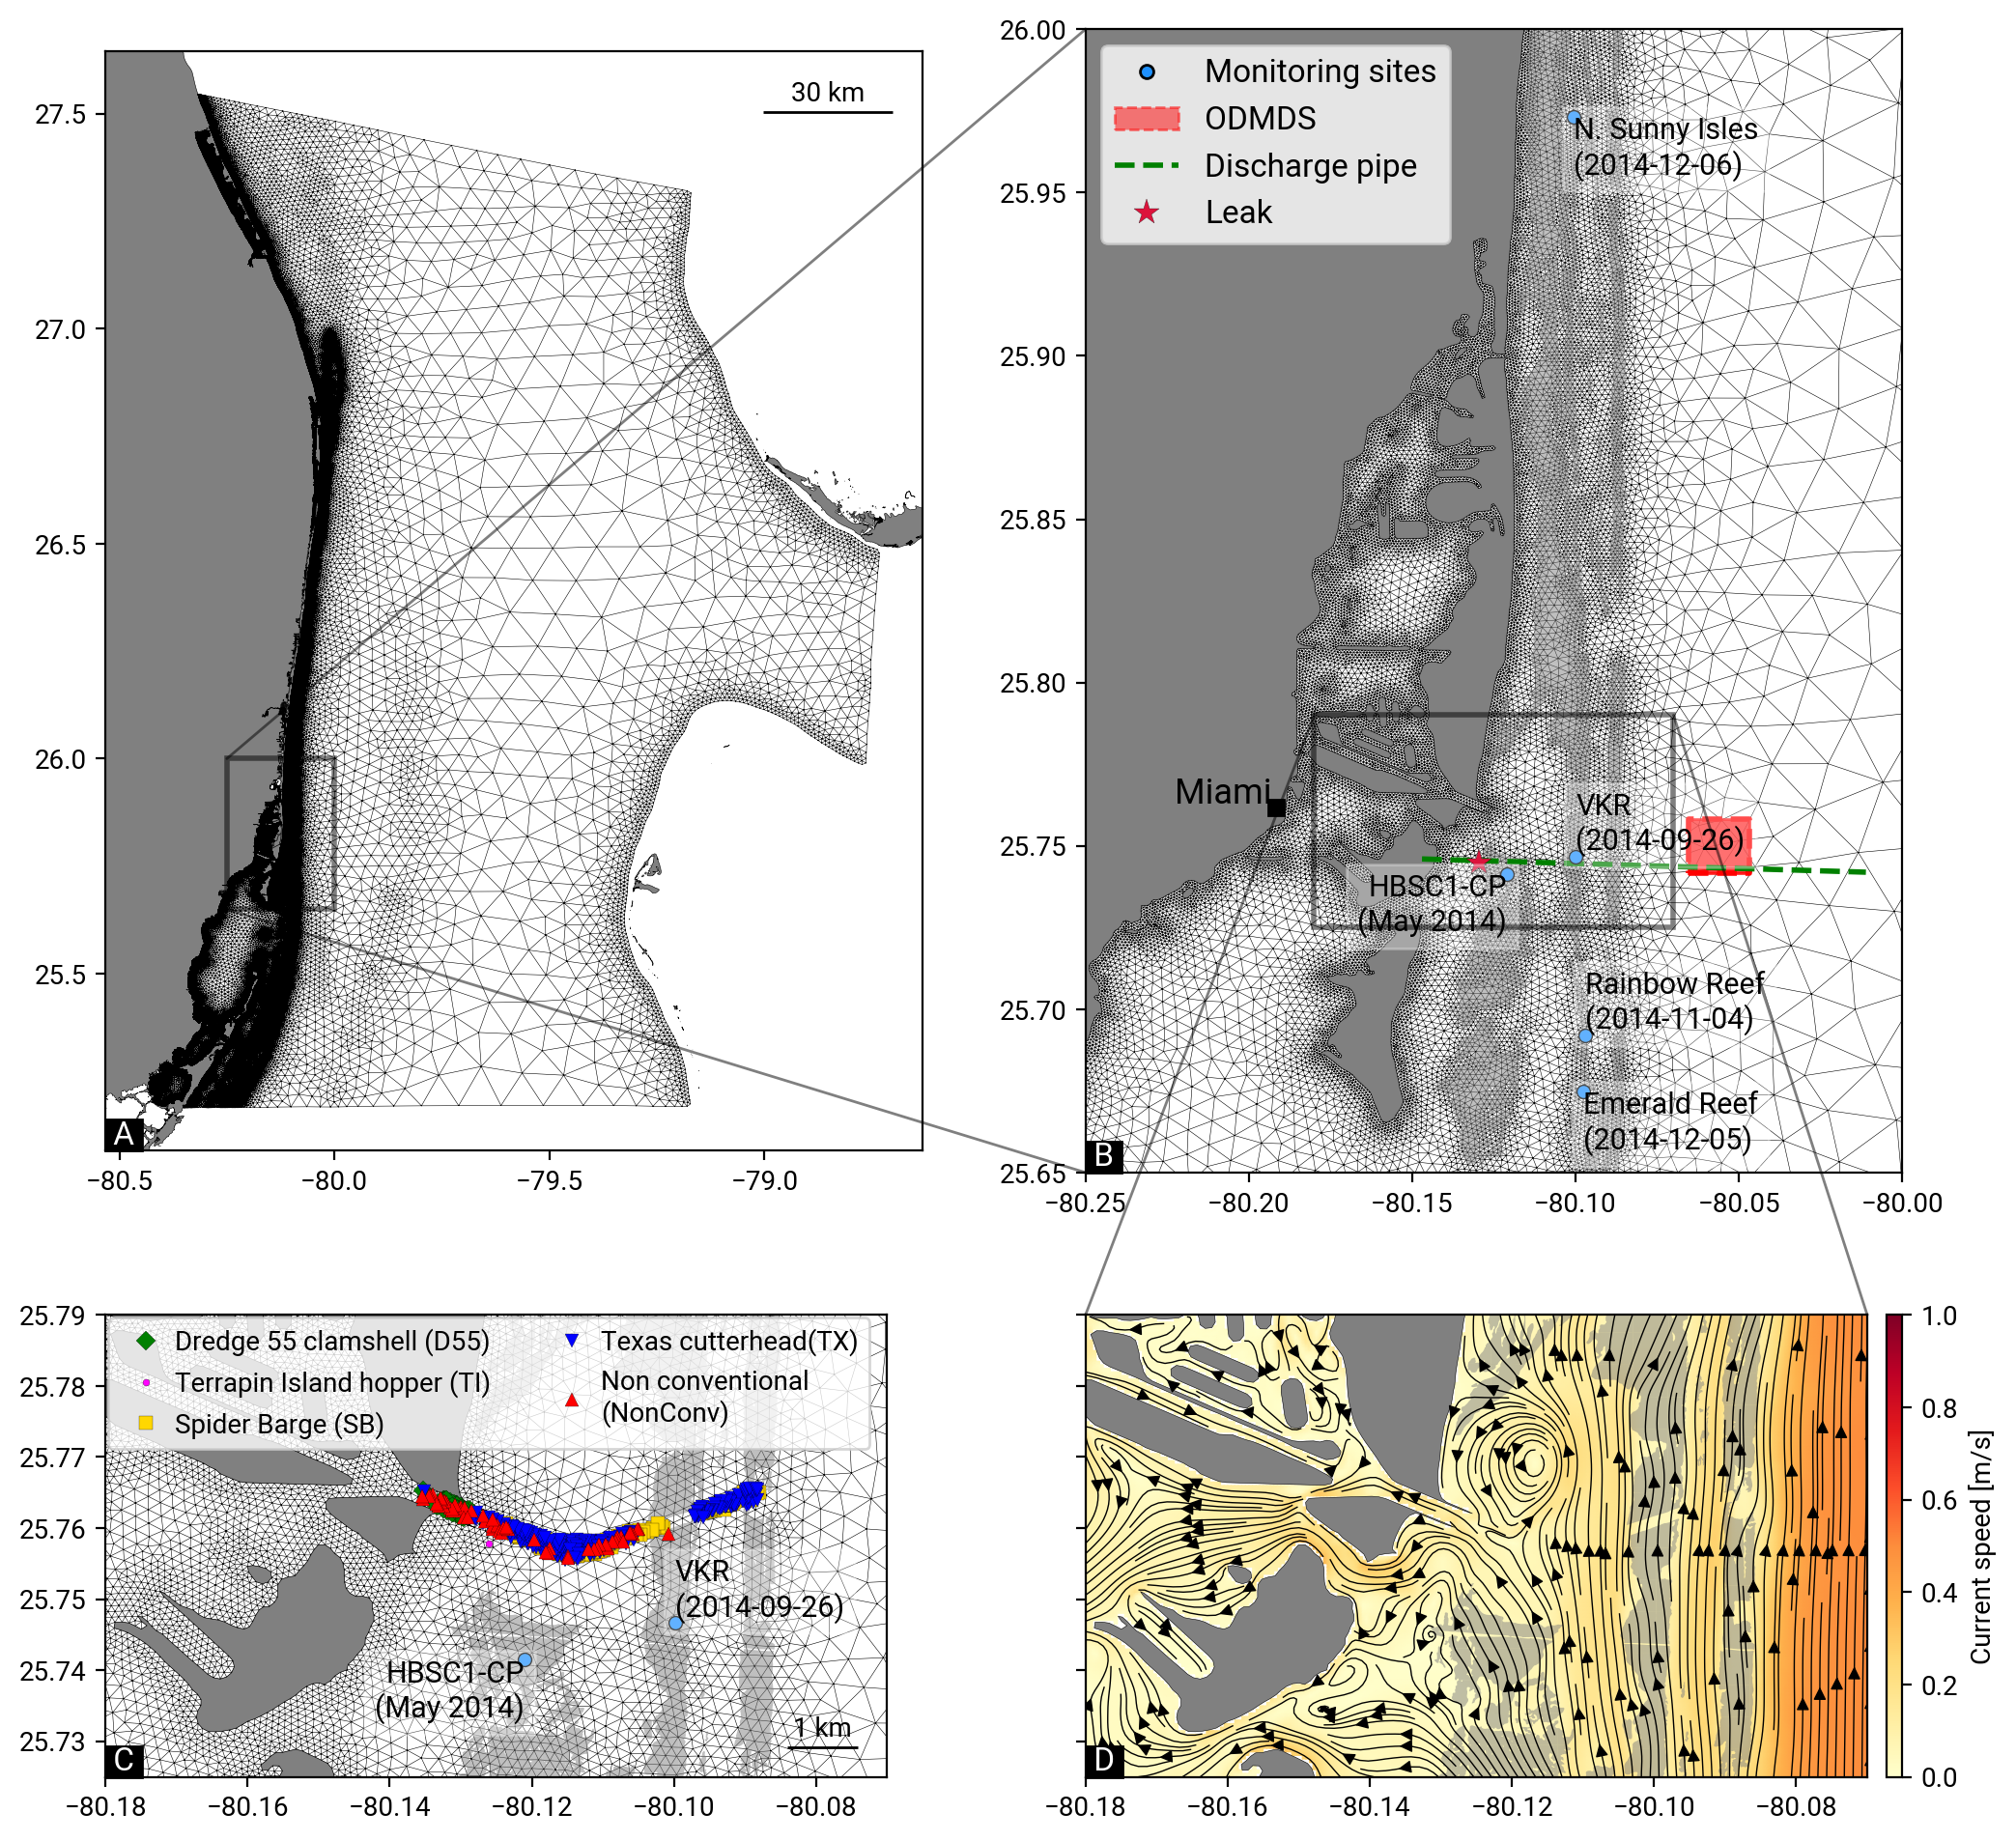
\includegraphics[width=\textwidth]{figures/fig_mesh_new.png}
    \caption{Model mesh (\textbf{A}) over the whole domain and (\textbf{B}) near the dredged channel. The mesh resolution reaches $\sim$100 m over the reefs (in light grey) and along the coasts (in dark gray). The coral reef monitoring sites are shown by light blue dots. The date of the first reported signs of SCTLD at these sites is given between brackets. The Ocean Dredge Material Disposal Site (ODMDS) is shown in red and the discharge pipe of the Miami Central Municipal WWTP in green. (\textbf{C}) Close-up view on the dredged channel. The locations of the different types of dredging that took place during the PortMiami expansion are shown by colored markers. (\textbf{D}) Snapshot of the modeled currents in the vicinity of the dredged channel. Small-scale flow features such as the acceleration of currents between reefs and islands are well reproduced by the model.}
	\label{fig:onset_mesh}
\end{figure}

Given the location of the monitoring sites where disease signs were observed during the dredging operations and the northward ocean circulation patterns that predominantly transport sediments in that direction, we considered an area of interest situated between Florida and the Bahamian Banks, and between 25.5$^\circ$N and 27.5$^\circ$N (Fig.~\ref{fig:onset_mesh}A). We simulated the hydrodynamics with the multiscale ocean model SLIM\footnote{\url{ https://www.slim-ocean.be}}. This model has already been extensively used and validated in the FCR \citep{frys2020fine,dobbelaere2020coupled,dobbelaere2022impacts,dobbelaere2022connecting}. SLIM uses an unstructured mesh whose resolution can be locally increased in order to accurately represent fine-scale flow features. The model resolution was defined by following the same approach as~\citep{dobbelaere2020coupled}. It reaches a resolution of $\sim$100 m over coral reefs and near the PoM to precisely represent the dredged channel (Fig.~\ref{fig:onset_mesh}B). The mesh is composed of $\sim$1.76$\times 10^5$ triangles and was generated with the seamsh\footnote{\url{https://pypi.org/project/seamsh/}} Python library, which is based on the open-source mesh generator GMSH \citep{geuzaine2009gmsh}. The model was run between October 15, 2013, and September 26, 2014, with a time step of 10 minutes to cover the whole dredging period prior to the observation of SCTLD at VKR by~\cite{precht2016unprecedented}. The modeled sea surface elevation and currents were exported every hour. Using such a fine mesh resolution, we simulated fine-scale details of the ocean currents, such as the flow acceleration between reefs and islands (Fig. \ref{fig:onset_mesh}D). Atmospheric forcings were obtained from the European Centre for Medium-range Weather Forecasts (ECMWF) ERA-5 dataset and currents were relaxed towards the operational Navy HYbrid Coordinate Ocean Model (HYCOM; \citealp{chassignet2007hycom}) following the approach of~\cite{dobbelaere2022impacts}. The modeled sea surface elevation was validated using tide gauge measurements from the National Data Buoy Center at stations 8722670 and 8723214, which are respectively located at Lake Worth Pier and Virginia Key (see~\ref{onset:validation}).

We then simulated the transport of sediments released by different dredging operations along the channel with a Lagrangian transport model forced by the simulated currents. Our sediment transport model is inspired by the Particle Transport Model (PTM), developed by the US Army Corps of Engineers \citep{macdonald2006ptm}. In this model, particles undergo a combination of horizontal and vertical motions. The vertical dynamics is mostly driven by gravity, with heavier particles sinking faster. Once they have settled, particles can be resuspended when shear stress exceeds the critical Schields parameter, as expressed by \cite{soulsby1997threshold}. The horizontal motion of the suspended particles is derived from the 2D model velocity by assuming a vertical log profile, hence yielding a quasi-3D approach. Furthermore, to account for the impact of wave-induced sediment motion, these current velocity were combined with surface Stokes drift velocity with Breivik's vertical profile \citep{breivik2016stokes}. Stokes drift's velocities were downloaded from Copernicus Marine Services's (CMEMS) Ocean Wave Reanalysis dataset \citep{cmems}. When sediment particles enter the near-bed zone, their horizontal velocity is greatly reduced and sediments are transported with the bed load.

As sediment dispersion is dependent on the grain size, we simulated the dispersal of five sediment classes to represent impacts of fine- to coarse-grained particles: (\textit{i}) 5-50 $\mu$m, (\textit{ii}) 50-100 $\mu$m, (\textit{iii}) 100-200 $\mu$m, (\textit{iv}) 200-300 $\mu$m, and (\textit{v}) 300-400 $\mu$m. We performed a  different simulation for each class, with the grain size randomly drawn from a uniform distribution over the corresponding size range. The density of each sediment particle was derived from its size using the formula of \cite{hamilton1982sound}. Furthermore, all particles were differentiated based on the type of dredge that produced them. Five types of dredge were considered in our modeling study: (\textit{a}) Texas cutterhead (TX), (\textit{b}) non-conventional dredging, \ie~TX with suction mechanism turned off (NonConv), (\textit{c}) Spider Barge (SB), (\textit{d}) Terrapin Island hopper (TI), and (\textit{e}) Dredge 55 clamshell (D55).

Dredging operations performed during the expansion of PoM were characterized in our dataset by a date, a location and a type of dredge (Fig. \ref{fig:onset_mesh}C). In the absence of information about the exact timing of the dredging, sediment particles were released from the dredging location during a whole day at a rate of 80 particles/hour in the model. To account for the motion of spider barges between the dredging and disposal sites, particles were released every 500 m along a straight line joining the dredging location to the ODMDS (see Fig. \ref{fig:onset_mesh}B) for every dredging operation labelled as SB.

We estimated the impact of the simulated sediment plumes on coral reefs by computing the turbidity and sedimentation generated by each type of dredging operations. Turbidity was derived from the concentration of suspended sediment particles. It is computed by counting the number of suspended particles within the cells of a regular 200 m $\times$ 200 m grid covering the entire computational domain. The modeled plumes were then compared with daily plume observations derived from satellite imagery by~\cite{cunning2019extensive}\footnote{Datasets available at \url{https://github.com/jrcunning/pom-dredge/}} following the methods of \cite{barnes2015sediment} at sites located within 15 km of the dredged channel. As in these two studies, we computed the simulated plume frequency by dividing the number of days during which sediment plumes occurred by the total number of simulated days for all grid cells. Sedimentation was quantified by computing the cumulated concentration of settled particles within the same grid as for turbidity. This cumulated concentration was normalized by the total numbers of simulated time steps and released particles. The normalized sedimentation indicator gives the averaged fraction of the total mass of particles released that settled in each grid cell by unit of area during the simulation. High sedimentation values indicate larger sediment deposition over a longer cumulated time.

We specifically assessed the potential impact of dredging operations at five monitoring sites where signs of coral disease were reported. Four of these sites are reefs where the disease was observed by~\cite{precht2016unprecedented} between Sept. and Dec. 2014. The fifth site is station HBSC1-CP, which was closely monitored throughout the expansion of PoM and where disease signs were already reported in May 2014 (\citealp{dial2017}; Fig. \ref{fig:onset_mesh}A, see~\ref{onset:appendice}). It remains however unclear if the disease observed at station HBSC1-CP was the SCTLD. The impact of dredging was assessed by identifying the dredging operations that produced sediment transported within 500 m of all five sites. We then computed the fraction of the sediment particles produced by these dredging operations that were actually transported within 500~m of the monitoring sites. The 500~m radius was chosen to match the scale of the 500~m $\times$ 500~m reef polygons used in the model \citep{dobbelaere2020coupled}. The resulting particle counts were then normalized by dividing them by the total number of sediment particles released by each dredging operation. Higher values of this indicator suggest a more significant impact of a specific type of dredging on the corresponding monitoring sites.

Additionally, we simulated the dispersal of dissolved pollutant particles backward in time from VKR and HBSC1-CP to identify sources of wastewater that could have affected these two sites. Ten particles were released from each site every 450 seconds between September 26, 2014, and October 15, 2013, for a total of $\sim$6.7$\times10^5$ particles per site. These simulations allowed us to assess whether wastewater leaking from the Miami Central District Municipal WWTP discharge pipe (Fig.~\ref{fig:onset_mesh}B) could have impacted HBSC1-CP and VKR, as suggested by \cite{gintert2019regional}. As leaking wastewater particles were expected to be positively buoyant (Precht, \textit{pers. comm.}, \emphc{not sure we should mention him here...}), there were advected backward in time by a combination of ocean currents and Stokes drift from CMEMS' Ocean Wave Reanalysis dataset. We then computed risk maps by counting the number of particle trajectories intersecting each cell of a 200 m $\times$ 200 m grid, following the same approach as~\cite{anselain2023qatar}. This number was normalized by the total number of released particles to obtain the probability for each grid cell to be a source of pollution that would reach the monitoring sites.
% Neutral buoyancy of wastewater loads was assumed as a limiting scenario for purposes of this study: observations \citep{bloetscher2014use,wanninkhof2005farfield} suggest that buoyant plumes may transport wastewater several kilometers under prevailing currents and winds in this region.
This probability was then integrated along the wastewater discharge pipe, modeled as a straight line between Miami Central District Municipal WWTP, located on Virginia Key, and the ocean discharge outfall located at 25$^\circ$44'31''N 80$^\circ$05'10''W \citep{koopman2006ocean}.

Finally, as previous studies showed evidence of waterborne transmission of SCTLD \citep{aeby2019pathogenesis, dobbelaere2020coupled,eaton2021measuring, meiling2021variable}, we assessed whether the disease could have been transmitted to VKR from other reefs affected by sediments from non-conventional dredging operations prior to September 2014. To evaluate this possibility, we computed monthly disease connectivity matrices following the methodology of \cite{dobbelaere2020coupled} during our simulated period. These connectivity matrices can be interpreted as large graphs whose vertices are 500 m $\times$ 500 m sub-reef polygons and whose edges represent disease connectivity pathways. Evaluating the possibility of disease propagation from sub-reefs affected by non-conventional dredging to VKR is therefore equivalent to evaluating the existence of pathways, \ie~sequences of connected vertices in the network starting from these sub-reefs and reaching VKR. As computing all possible pathways is not computationally tractable, we limited ourselves to the computation of shortest paths from the affected reefs to VKR. This was performed using the function \texttt{get\_all\_shortest\_paths} of the Python \texttt{python-igraph} package \citep{csardi2006igraph}. Such a function requires the definition of a weight $w_{ij}$ for the edge connecting reef $i$ to reef $j$. We chose $w_{ij} = 1-\tilde{C}_{ij}$, where $\tilde{C}_{ij}$ is the probability of disease propagation from reef $i$ to reef $j$ computed following the approach of \cite{dobbelaere2020coupled}, so that `shorter' edges of the networks (\ie~connectivity pathways with smaller weights) correspond to connections with a larger disease propagation probability. The probability of a given path was then defined as the mean connection probability of the edges composing this path.


%%%%%%%%%%%%%%%%%%%
% --- RESULTS --- %
%%%%%%%%%%%%%%%%%%%
\section{Results}

% FIGURE 2 - PLUMES
% Plume frequency
% HSBC1-CP:4.14
% VKR: 0.32
% N. Sunny Isles: 19.43
We simulated sediment plumes for all dredging operations across five sediment size classes, with grain sizes ranging from 5 to 400 $\mu$m. Of these, only the grain sizes between 5 and 50 $\mu$m generated plumes that were consistent with the observations reported by~\cite{barnes2015sediment} and~\cite{cunning2019extensive} (Fig.~\ref{fig:onset_depo}A). For coarser grain sizes, particles settled in the direct vicinity of the dredged channel. The suspended sediments were then only observed offshore, closer to the Florida Current, where the current velocity was sufficiently strong to prevent deposition (Fig. \ref{fig:onset_depo}B). This suggests that the observed turbidity was mostly due to fine silts. With grain sizes of 5-50 $\mu$m, the modeled occurrence of plumes  within 15 km of the dredged matched the presence/absence data of~\cite{cunning2019extensive} in 80.5\% of cases and the total area where plumes were observed was about 205 km$^2$, consistent with the $\sim$228 km$^2$ estimated by~\cite{barnes2015sediment}. The simulated suspended sediment plumes mostly occurred north of the dredged channel, as particles were driven northward under the action of shelf currents influenced by winds and the Florida Current. The highest simulated plume frequency was about 60\% and was found within a region of about 1.5~km $\times$ 1.5~km north of the dredged channel and just next to Miami Beach (Fig.~\ref{fig:onset_depo}A). Plume frequencies locally reaching 30-40\% were observed within 4~km north of the dredged channel, between the coasts and the inner reef line. Suspended sediment plumes were observed during $0.32$~\% of simulated days at VKR site, $4.14$ \% at HBSC1-CP and $19.43$ \% at N. Sunny Isle. Similarly to~\cite{cunning2019extensive}, we found a positive correlation between plume frequency and sediment deposition, with a Pearson correlation coefficient of 0.29.

% \begin{table}
%     \centering
%     \begin{tabular}{|l|cccc|}
%         \hline
%          & Threshold         & Accuracy & False positive  & False negative \\
%          & [particles/m$^2$] & [\%]     & [\%]            & [\%]  \\
%         \hline
%         5-50 $\mu$m    & 21 & 86.678 & 2.912 & 10.410 \\
%         50-100 $\mu$m  & 20 & 83.058 & 8.525 & 8.417 \\
%         100-200 $\mu$m & 30 & 84.814 & 7.133 & 8.053 \\
%         200-300 $\mu$m & 18 & 84.459 & 7.988 & 7.553 \\
%         300-400 $\mu$m & 13 & 84.615 & 8.140 & 7.244 \\
%         \hline
%     \end{tabular}
%     \caption{Validation of the modeled presence of plumes against plume observations from satellite imagery. Overall, the model agrees well with observations}
%     \label{tab:onset_val}
% \end{table}

\begin{figure}
	\centering
	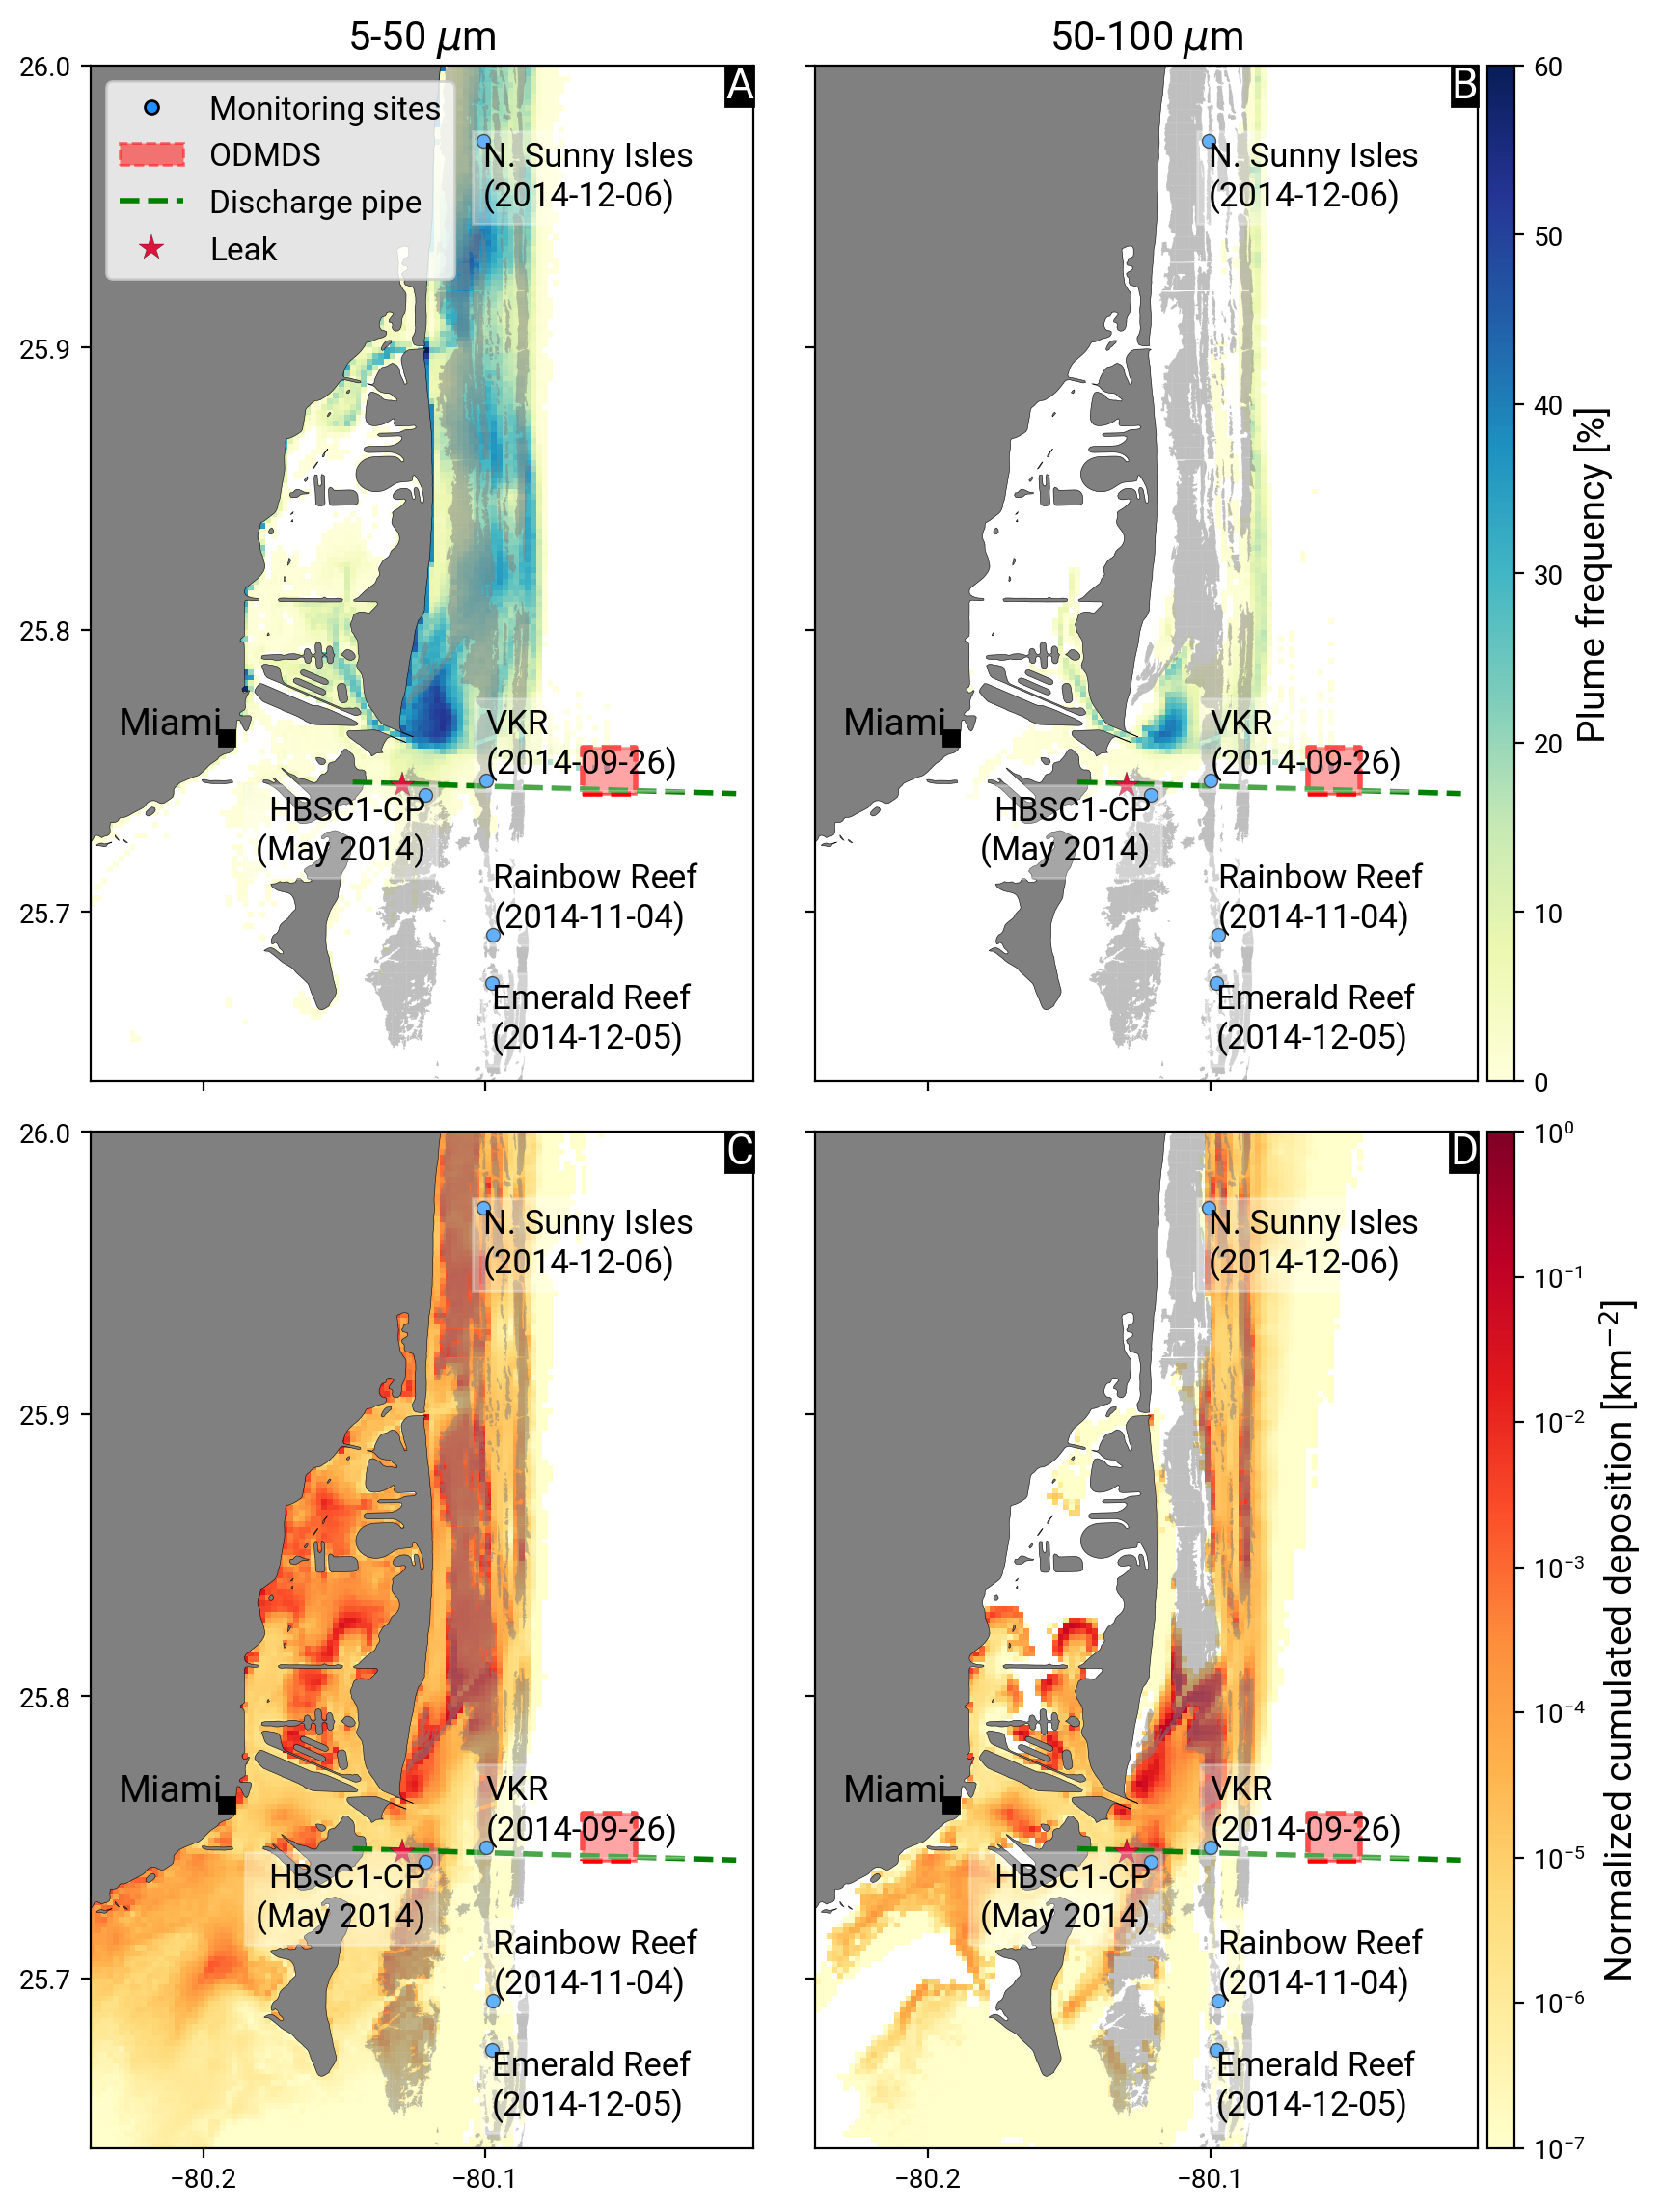
\includegraphics[width=.9\textwidth]{figures/fig2_stokes4_symmetrical.png}
    \caption{Suspended sediment plume frequency for grain size in the range 5-50~$\mu$m (\textbf{A}) and 50-100~$\mu$m (\textbf{B}). The averaged concentration of deposited sediments are shown for grain sizes more likely to carry the disease: 5-50~$\mu$m (\textbf{C}) and  50-100~$\mu$m (\textbf{D}). Most modeled turbidity and sedimentation occurred north of the dredged channel.}
	\label{fig:onset_depo}
\end{figure}

% FIGURE 2 - DEPOSITION
% Site           | Class 1 |  Class 2
% VKR            | 3.23e-6 | 7.63e-6
% HBSC1-CP       | 8.64e-4 | 1.386e-3
% N. Sunny Isles | 2.25e-4 | 5.72e-4
% Rainbow Reef   | 4.4e-7  | NA
% Emerald Reef   | 4.53e-9 | NA
Deposition results are shown for grain sizes between 5 and 100 $\mu$m, corresponding to silts and very fine sand, which are more likely to carry organic matter and therefore more likely to carry SCTLD agents \citep{erftemeijer2012environmental}(Fig.~\ref{fig:onset_depo}C,D). Sedimentation mostly occurred on reefs located north of the dredge channel, although some sediment particles deposited along the coastlines of Virginia Key, Key Biscayne and Miami for all modeled grain sizes. For grain sizes finer than 50~$\mu$m, sediments mostly settled on inshore reefs and along coastlines, while sedimentation mostly took place on offshore reefs for grain size coarser than 50~$\mu$m. Furthermore, sediment particles finer than 50 $\mu$m were deposited further south and west, covering the entire area between mainland Florida and the reef line. On average, the fraction of all sediments released depositing at VKR, HBSC1-CP and N. Sunny Isles was respectively $3.23\times10^{-6}$ km$^{-2}$, $8.64\times10^{-4}$ km$^{-2}$ and $2.25\times10^{-4}$ km$^{-2}$ for grain sizes of 5-50 $\mu$m, and $7.63\times10^{-6}$ km$^{-2}$, $1.39\times10^{-3}$ km$^{-2}$ and $5.72\times 10^{-4}$ km$^{-2}$ for grain sizes of 50-100 $\mu$m. The deposition at these two sites therefore decreased with increasing grain sizes. Additionally, the fraction of the total particle mass depositing at Rainbow Reef and Emerald Reef was respectively $4.4\times10^{-7}$ km$^{-2}$ and $4.53\times10^{-9}$ km$^{-2}$ for grain sizes of 5-50 $\mu$m, while no sedimentation occurred at these sites for grain sizes of 50-100 $\mu$m.

% FIGURE 3
Sediment particles with grain sizes of 5-50~$\mu$m and 50-100~$\mu$m, released by 99\% and 83\% of all simulated dredging operations respectively, reached N. Sunny Isles (Fig.~\ref{fig:onset_bar}). This makes it the reef site most impacted by the simulated dredging operations among the five sites considered here. HBSC1-CP was the second most impacted site, affected by 43\% and 35\% of the dredging operations involving grain sizes of 5-50~$\mu$m and 50-100~$\mu$m, respectively. VKR was the third most impacted site, receiving sediments from 12.4\% and 4.6\% of the dredging operations with grain sizes of 5-50~$\mu$m and 50-100~$\mu$m, respectively. Lastly, Rainbow Reef and Emerald Reef were each impacted by less than 4.5\% and 0.5\% of the dredging operations for grain sizes of 5-50~$\mu$m and 50-100~$\mu$m, respectively. More than 90\% of the modeled sediment particles were not transported within 500 meters of the reef sites, and the proportion of particles reaching the monitoring sites decreased as grain sizes increased. Despite this, N. Sunny Isles, VKR, and HBSC1-CP were all affected by fine sediments from non-conventional dredging operations. Specifically, when considering these operations, VKR, HBSC1-CP, and N. Sunny Isles were impacted by 1.17\%, 4.37\%, and 14.80\% of the sediments released for grain sizes of 5-50~$\mu$m, respectively, and by 0.38\%, 2.19\%, and 3.36\% for grain sizes of 50-100~$\mu$m. However, since non-conventional dredging is expected to release more sediments into the water column than conventional one, where dredged material is collected, these relative metrics may underestimate the true impact of the non-conventional dredging operations.

\begin{figure}
	\centering
	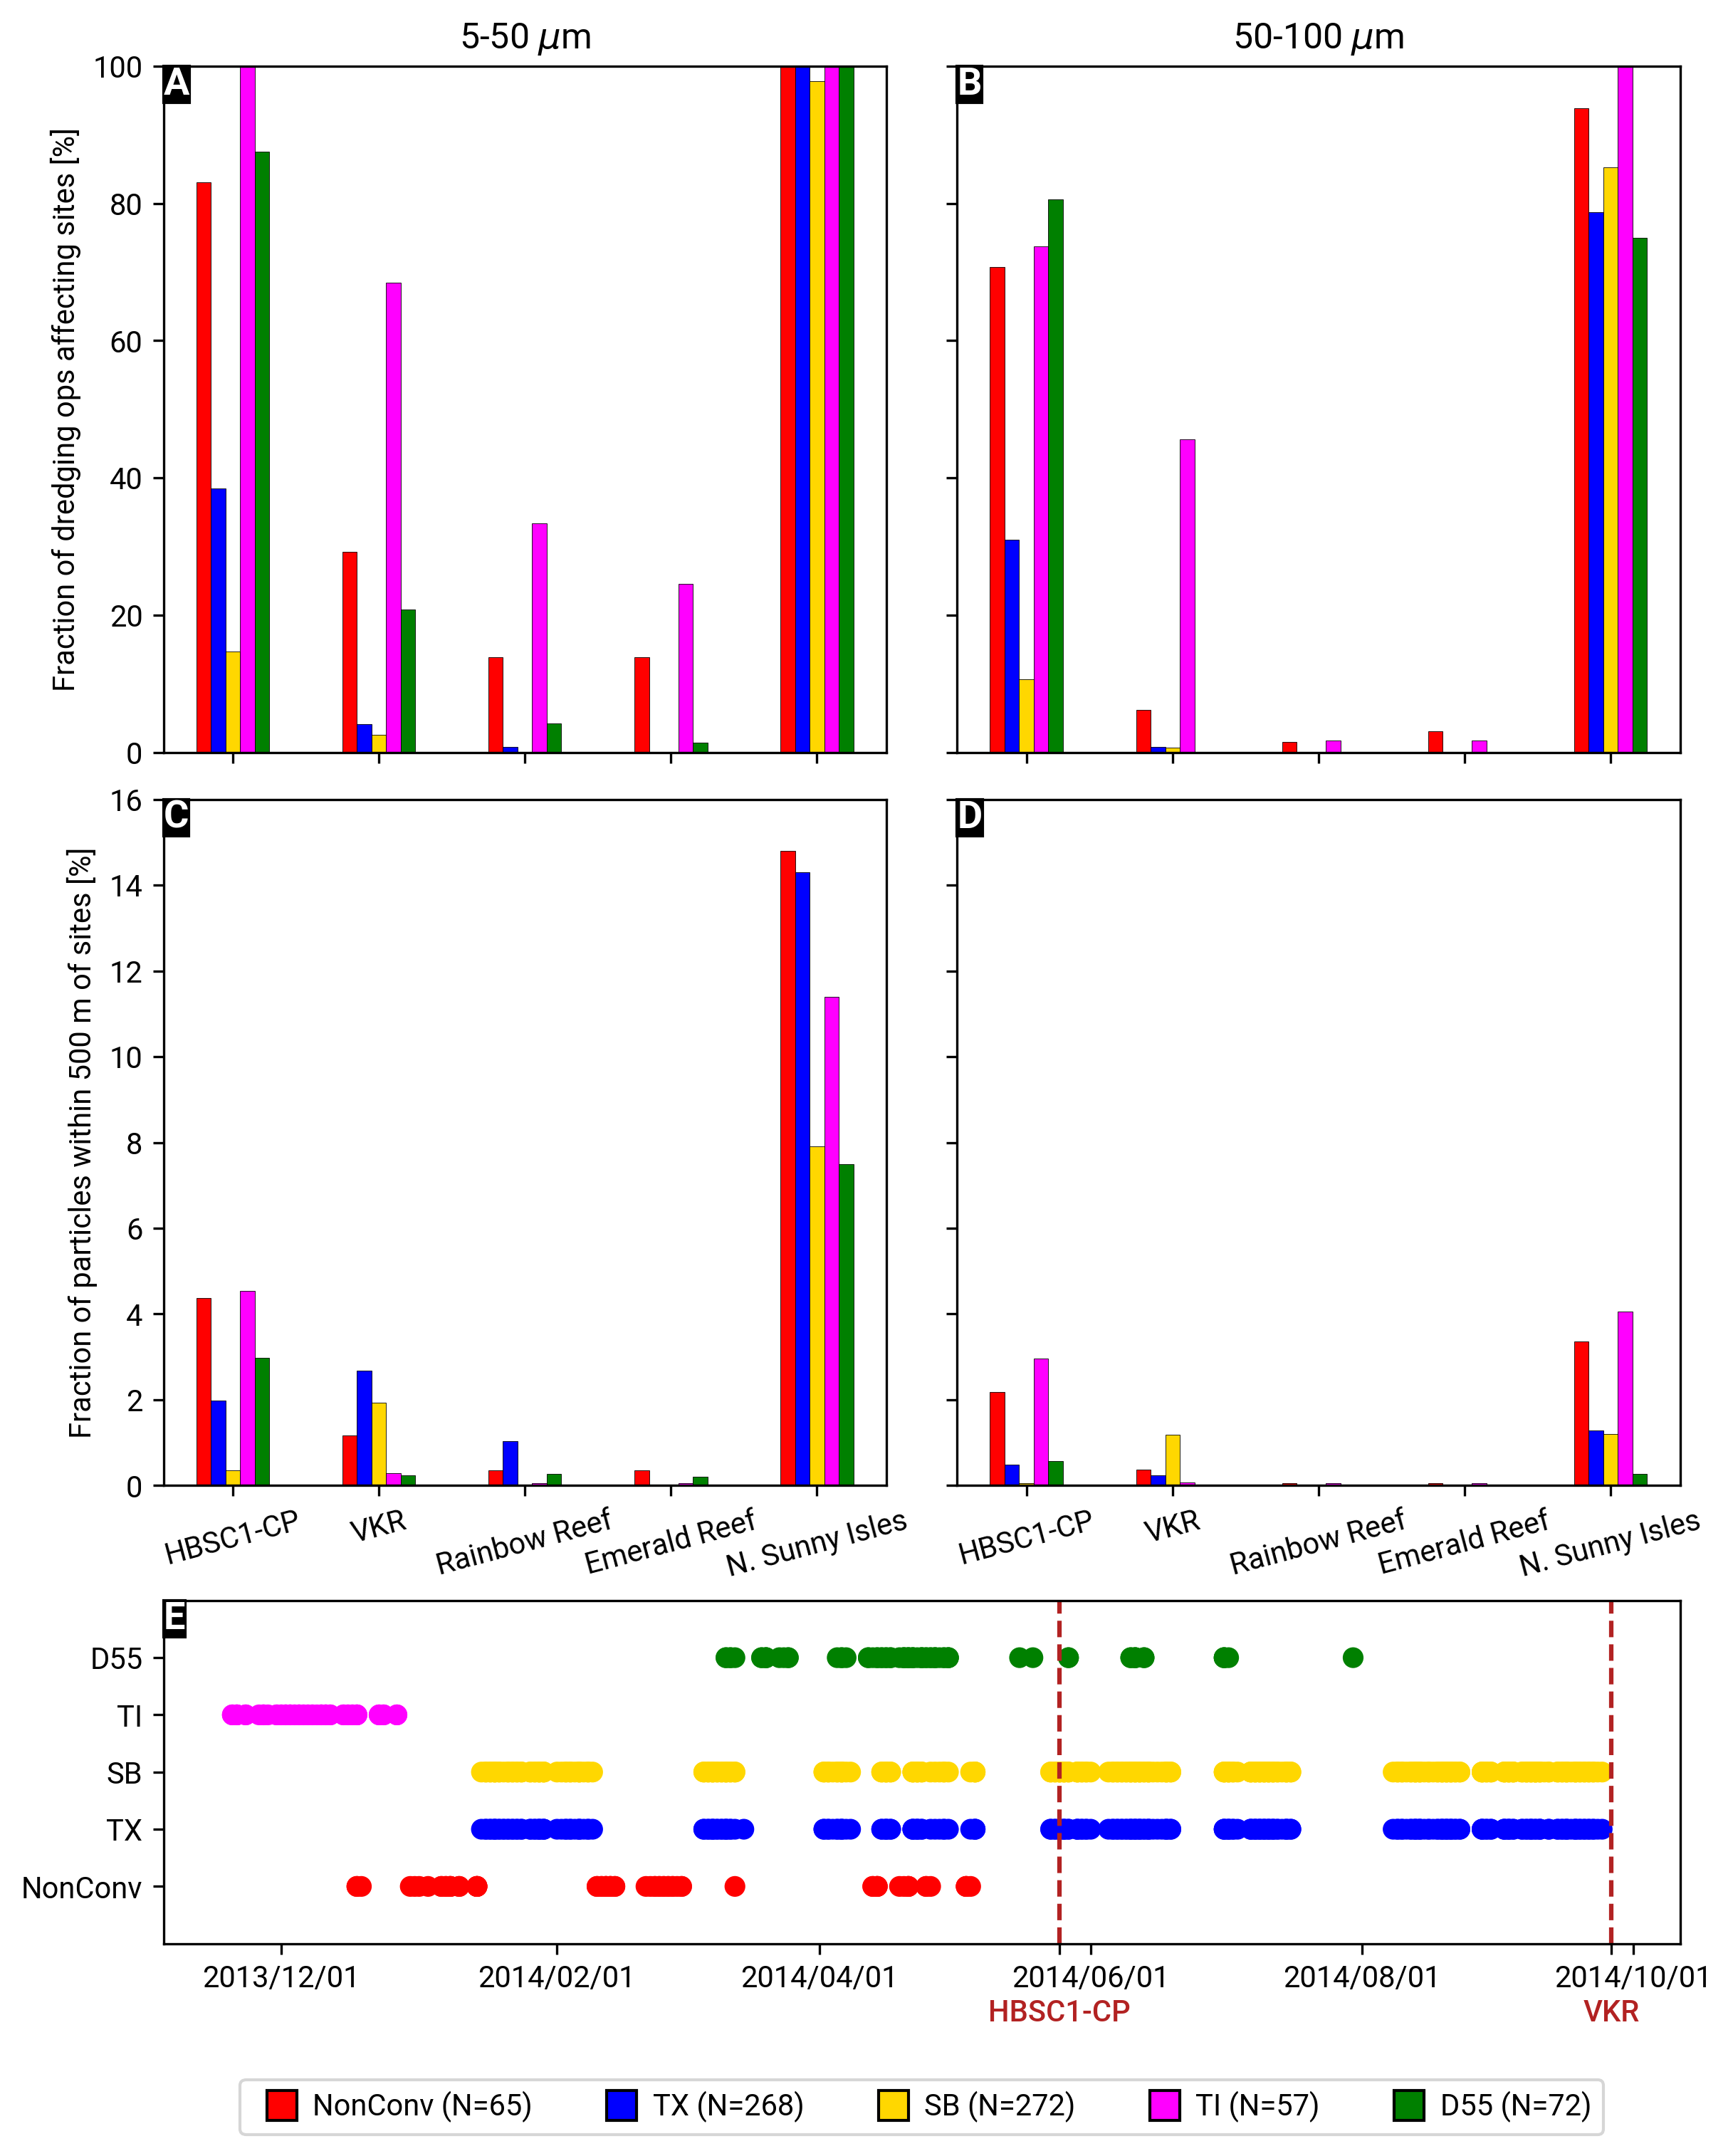
\includegraphics[width=.85\textwidth]{figures/aggregated_stokes4_v3_500m_timeline_rel.png}
	\caption{Fraction of simulated dredging operations producing sediment particles that were transported within 500~m of HBSC1-CP, VKR and N. Sunny Isles for grain sizes of (\textbf{A}) 5-50 $\mu$m  and (\textbf{B}) 50-100 $\mu$m. Fraction of the sediment particles produced by these operations transported within 500~m of HBSC1-CP, VKR and N. Sunny Isles for grain sizes of (\textbf{C}) 5-50 $\mu$m  and (\textbf{D}) 50-100 $\mu$m. \textbf{E}: Temporal distribution of the simulated dredging operations. The dates of the first reported disease signs at HBSC1-CP and VKR site are shown with dotted dark red vertical lines. The total number of simulated dredging operations (N) is given between brackets for each dredging type. N. Sunny Isles was the most affected site. All sites were impacted by non-conventional dredging for the two considered grain sizes}\label{fig:onset_bar}
\end{figure}

% FIGURE 4
When analyzing wastewater pollution by backtracking particle from HBSC1-CP and VKR, we see that the most likely sources of pollution impacting these sites were located within narrow "cones" directly south of the sites (see red parts of the plumes in Fig.~\ref{fig:backtrack}). Within these cones, the probability of pollutants reaching the sites decreased southward: it fell below 30\% at a distance of 300 m, below 10\% between 1 and 1.5 km, below 5\% at 3 km, and below 1\% at 15 km from the sites. Outside these cones, the likelihood of pollutants reaching VKR and HBSC1-CP rapidly dropped below 1\%. By integrating the probability of pollutant arrival along the wastewater discharge pipe, we determined that the likelihood of pollutants leaking from the pipe and reaching HBSC1-CP (located south of the pipe) was below 5\% within 2 km of the site, and then fell below 1\%. Conversely, the probability of leaking pollutants reaching the VKR site (located north of the pipe) was as high as 40\% at the site's location, but dropped below 1\% within 500 m of the site. This indicates that a leak affecting HBSC1-CP is unlikely, and VKR would only be affected if the leak occurred within 500 m of the site.

\begin{figure}
    \centering
    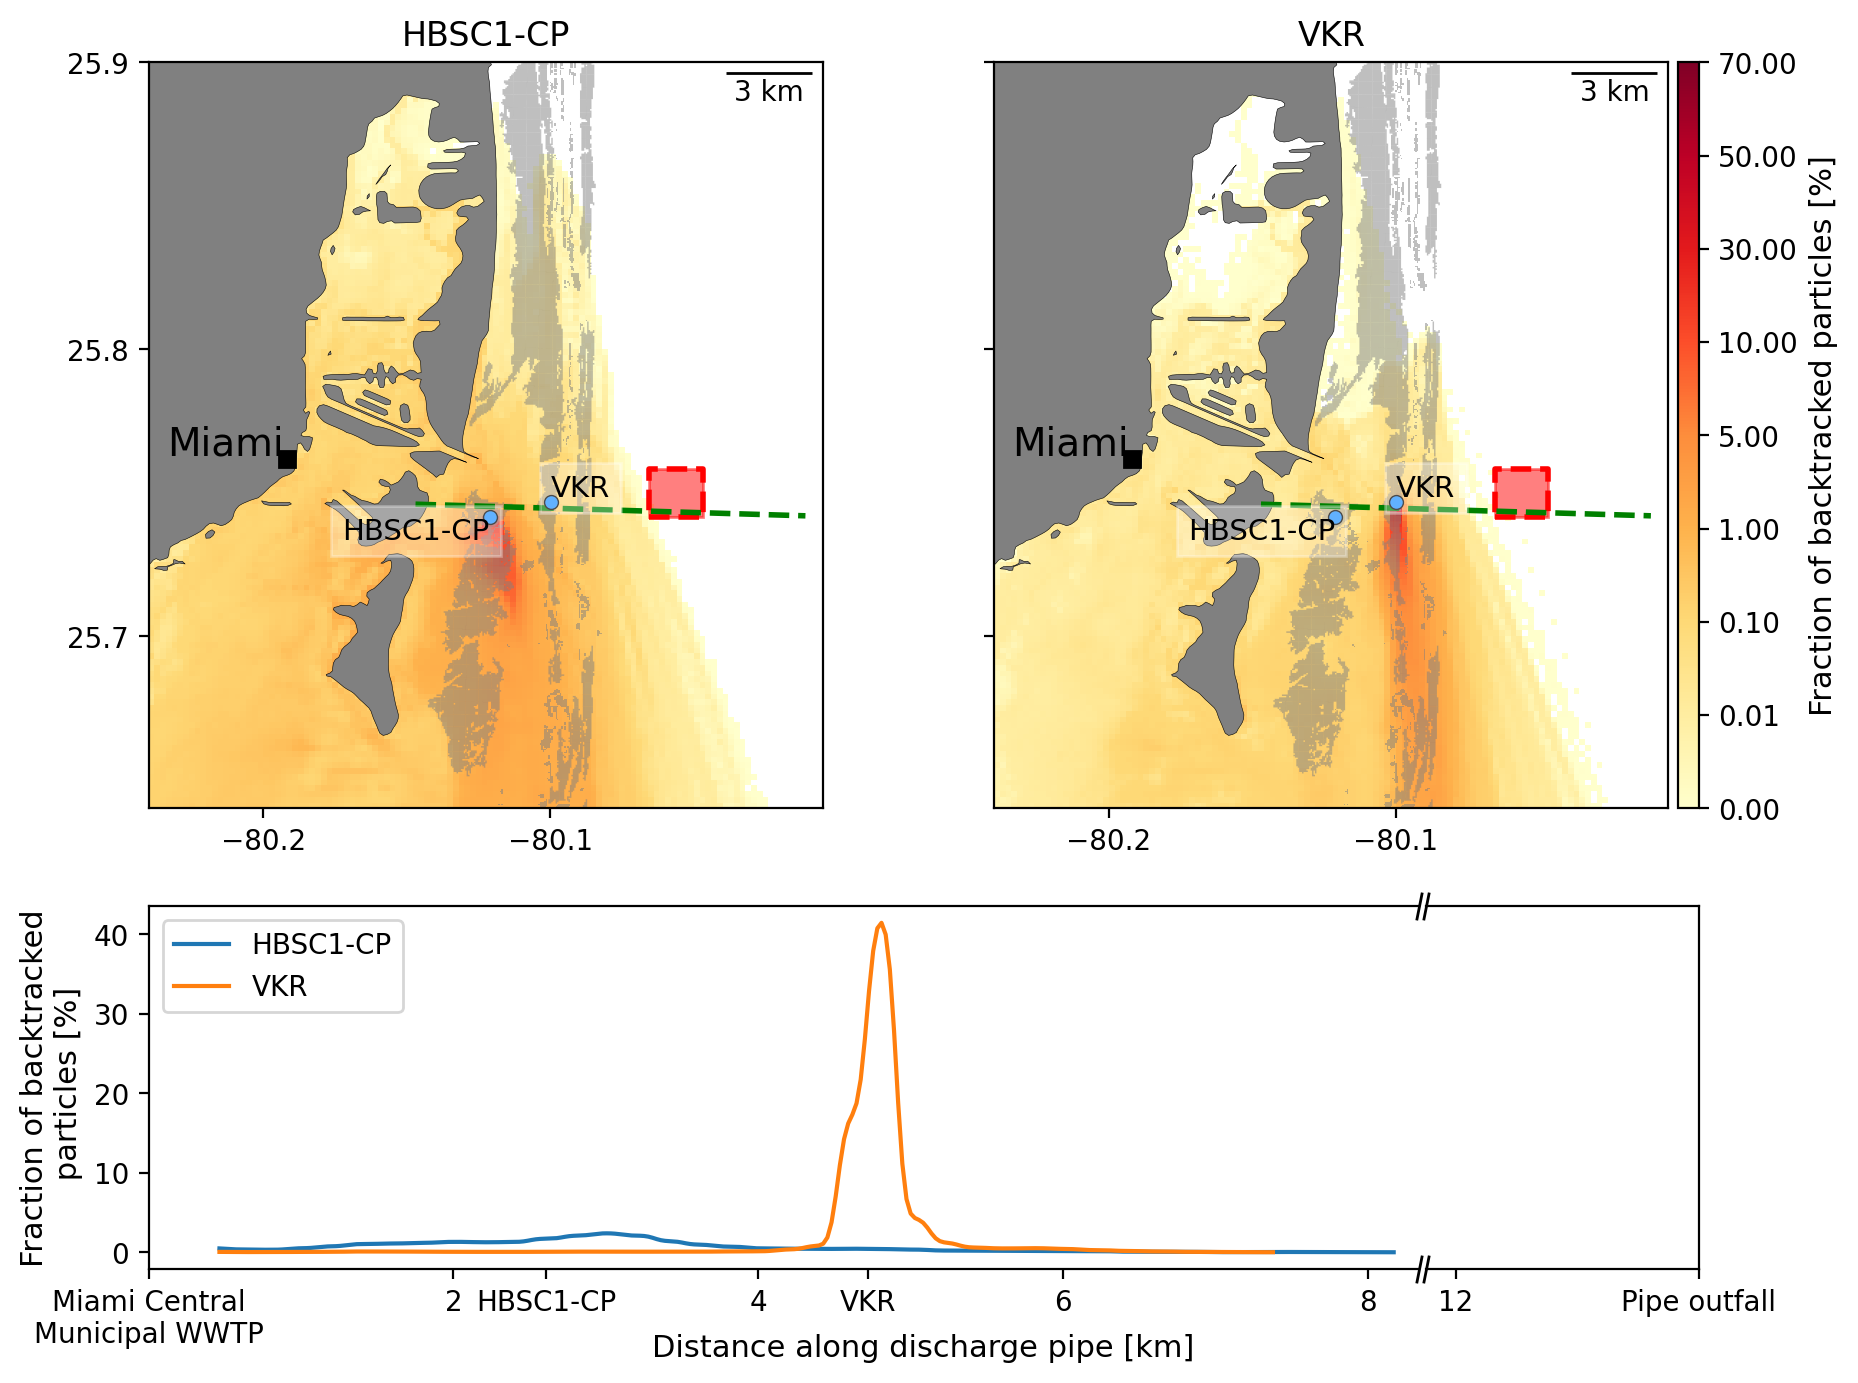
\includegraphics[width=.98\textwidth]{figures/fig_proba_stokes_v2.png}
    \caption{Spatial distribution of the probability to be a source of positively buoyant pollutants reaching HBSC1-CP (\textbf{top left}) and VKR (\textbf{top right}). \textbf{Bottom}: Integration of this probability along the discharge pipe of Miami Central District Municipal WWTP, which was reported to leak in 2017. Most likely sources of pollutants were located within a few kilometers south of HBSC1-CP and VKR. In the top panels, the Ocean Dredge Material Disposal Site (ODMDS) is shown in red and the discharge pipe of the Miami Central Municipal WWTP in green.}
    \label{fig:backtrack}
\end{figure}

% FIGURE 5
We then evaluated the likelihood that reefs affected by non-conventional dredging could become infected and subsequently transmit the disease to VKR. To do this, we calculated all the shortest paths from these impacted reefs to VKR using modeled monthly disease connectivity networks from May to September 2014 (Fig.~\ref{fig:onset_path}). These pathways included HBSC1-CP, where potential signs of the disease were reported in May 2014. Our results reveal that there were connectivity pathways to VKR in each of the months from May through September 2014, indicating a continuous potential for disease spread from the affected reefs to VKR during this period. Southern intermediary reefs were consistently needed as stepping stones for this disease transmission, suggesting that it might have taken several months for the disease agents to reach VKR from the reefs influenced by non-conventional dredging. However, the structure of these connectivity pathways remained relatively consistent throughout May-Sept. 2014, indicating persistent favorable conditions for disease propagation to VKR.
% * <thomas.dobbelaere@uclouvain.be> 13:26:22 18 May 2022 UTC+0200:
% Lew: should be justify why no observation of SCTLD at VKR in the meantime

\begin{figure}
	\centering
	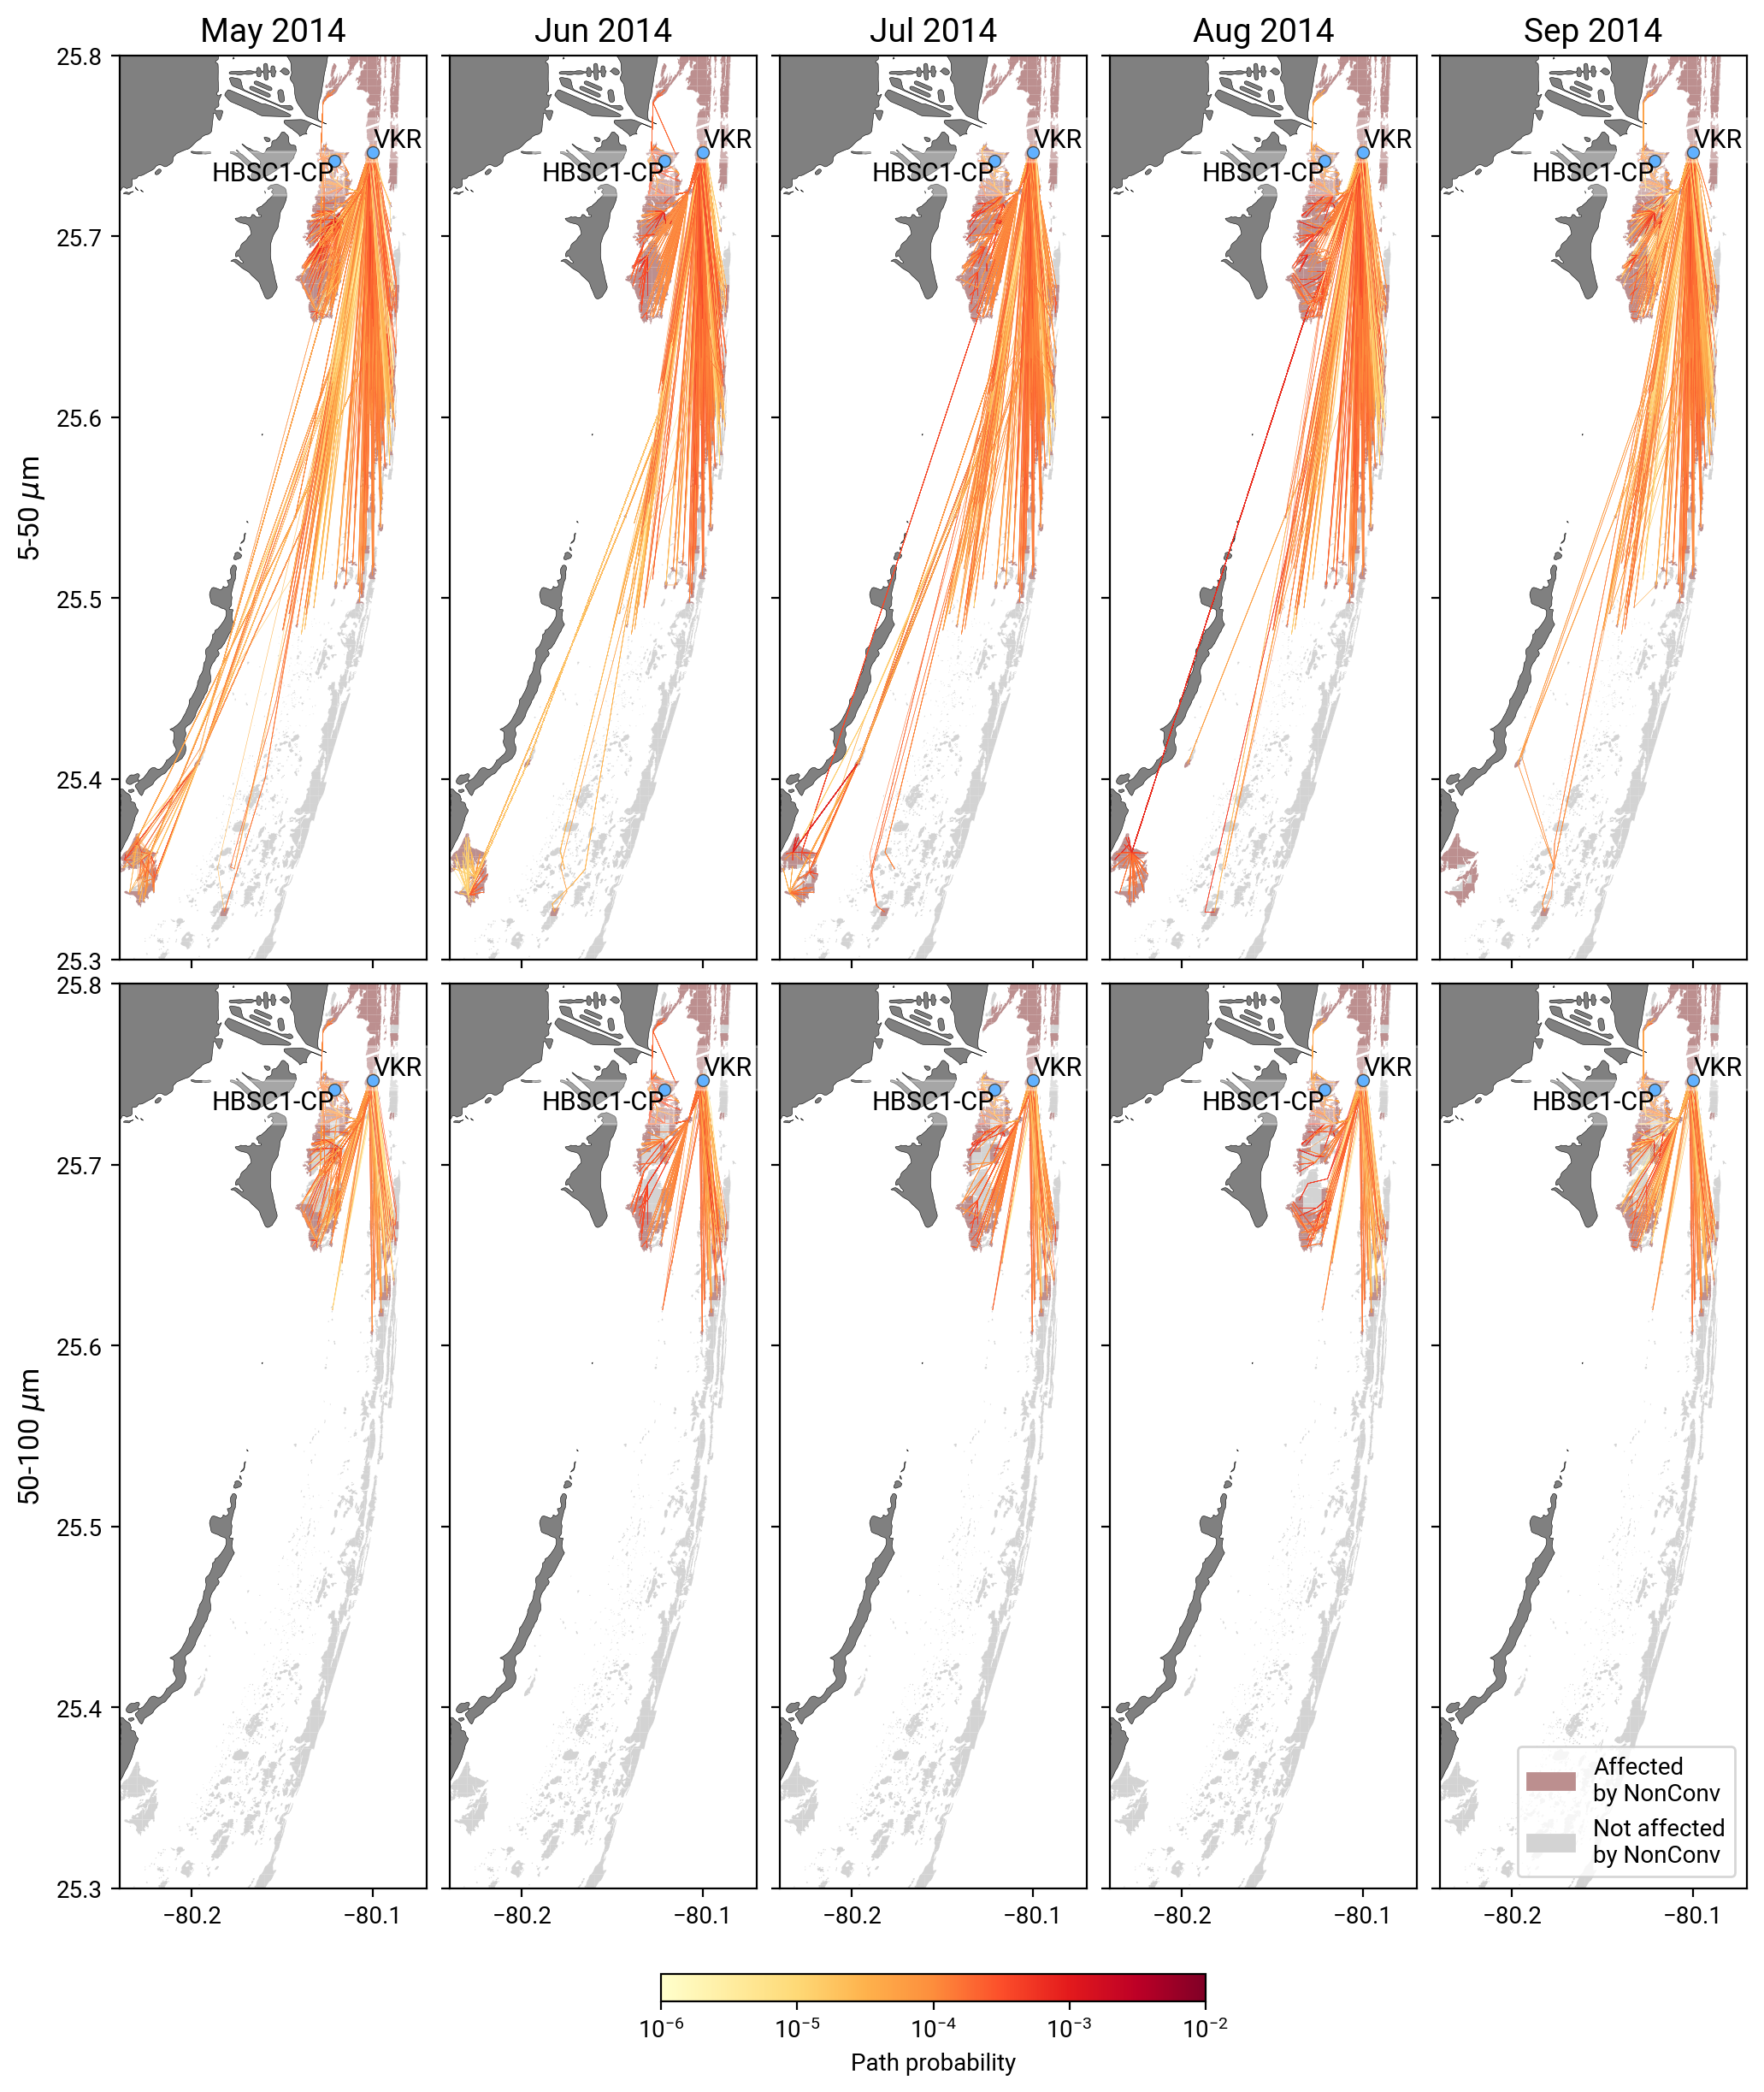
\includegraphics[width=\textwidth]{figures/figure_new_shortest_paths.png}
    \caption{Shortest path distributions from all the reefs affected by non-conventional dredging operations to the monitoring site near Virginia Key (VKR) for the monthly disease connectivity networks of May to September 2014. Southern intermediary reefs were always needed as stepping stones for the propagation of the disease to VKR.}
	\label{fig:onset_path}
\end{figure}

% === DISCUSSION === %
\section{Discussion}

% Importantly, this study only considered two possibilities that may have contributed to the SCTLD outbreak: dredging activities and a pollutant leak. Among these two options, there is more support for dredging than a pollutant leak because the probabilities that pollutants reached sites where SCTLD was possibly first observed were lower than the probabilities of sediment from dredging reaching the same sites; no leaks were reported in this early period; and the area was monitored well. Additionally, we cannot rule out HSCB1-CP as a potential source for the SCTLD outbreak over VKR because connectivity matrices demonstrate SCTLD could have reached VKR via stepping stones; and HSCB1-CP would have received more sediment from dredging than VKR if dredging is in fact the causative agent.”

% SUMMARY
Employing a high-resolution quasi-3D sediment transport model, we successfully reproduced sediment dynamics that align with plume observations from satellite imagery and in situ sediment deposition data at selected sites. The best agreement was obtained for grain sizes in the range 5-50 $\mu$m, suggesting that dredging operations mostly released fine-grained sediments, which include the very fine "rock flour" produced by non-conventional rock-chopping operations. Those sediments predominantly drifted northward, over several kilometers, under the influence of the Florida Current. The impact of dredging on southern sites such as Rainbow Reef and Emerald Reef was minimal, whereas up to 12\% of the dredging activities directly influenced VKR, where the initial outbreak of SCTLD was reported in September 2014 \citep{precht2016unprecedented}. Additionally, our analysis suggests that the VKR site was unlikely to be affected by wastewater leaking from the Miami Central District Municipal WWTP discharge pipe unless the leakage occurred within 500 meters of the site. Notably, signs of a disease -- though not definitively identified as SCTLD -- were observed at HBSC1-CP prior to September 2014, coinciding with both sediment plumes and deposition documented in our simulations. Moreover, monthly disease connectivity networks revealed that disease agents could have spread from reefs affected by non-conventional dredging to VKR via multistep connectivity pathways.

% LARGE IMPACT OF DREDGING
Our study confirms previous findings on the extensive impacts of the PoM expansion. Echoing \cite{barnes2015sediment}, the sediment plumes simulated with our model have a total surface area of about 205 km$^2$. Additionally, our model achieved an 80.5\% accuracy in replicating the presence or absence of plumes within 15 km of the dredged channel, as detailed by \cite{cunning2019extensive}. This high level of accuracy was specifically observed for grain sizes ranging from 5 to 50 $\mu$m. This suggests that the silt and clay-like "rock flour" materials, resulting from unconventional rock chopping, were the primary contributors to the turbidity during dredging, aligning with findings from previous research \citep{storlazzi2015influence,fourney2017additive}. Despite this congruence, our model predicted a northward shift in plume distribution compared to these earlier studies, possibly due to our method focusing solely on suspended sediment concentration, whereas turbidity is influenced by various local factors including phytoplankton water content and organic matter \citep{gray2000comparability,thackston2000improved}. Consistent with \cite{cunning2019extensive}, our results identified a positive correlation between sedimentation rates and plume frequency. Significantly, the regions with the highest cumulative sediment deposition were predominantly over coral reefs, suggesting that the PoM expansion adversely affected coral populations across a broad area through increased turbidity and sedimentation. \emphc{Say that the impacted area extends over several km and is hence much larger than the area initially considered for coral monitoring and subsequent restoration?} The sediment primarily settled on nearshore reefs with finer grain sizes and on offshore reefs with coarser grains. This sedimentation could be particularly detrimental to offshore coral reef populations, which are generally less adapted to sediment exposure compared to their inshore counterparts \citep{wolanski2005fine}.

% LIMITATION ABOUT AMOUNT OF RELEASED SEDIMENTS
A limitation of our study is that conventional and non-conventional dredging operations are treated in the same way in the model. For all dredging types, sediment particles were released at the same rate. Although conventional dredging was reported to release fine-grained sediments in the water column through dewatering and barge overflow \citep{jones2016assessing}, the quantity of dredged material lost in the water was limited by the use of pumping mechanisms. In contrast, for non-conventional dredging, the suction mechanism was turned off, causing all chopped rock particles to be released in the water column. The numbers of particles reaching the monitoring sites were therefore likely underestimated for non-conventional dredging operations. However, the fractions given in Fig. \ref{fig:onset_bar}C,D remain valid as they are relative to the total amount of sediment released in the water column for each type of dredging operation. When considering the simulated sediment plumes with the finest grain sizes, VKR, HBSC1-CP and N. Sunny Isles were respectively affected by 29\%, 83\% and 100\% of the non-conventional dredging operations that took place between December 2013 and May 2014. Furthermore, HBSC1-CP exhibited the highest deposition of sediments produced by non-conventional dredging. These sediment particles therefore had a higher probability to settle and to be in direct contact with corals. In addition to smothering corals and diverting their energy through sediment removal \citep{erftemeijer2012environmental}, these settled sediments spend more time in direct contact with the corals and might therefore yield a stronger disease transmission potential.

% The coral reefs of N. Sunny Isles appeared to be highly exposed to fine-grained sediments produced by dredging (Fig. \ref{fig:onset_bar}). Furthermore, the non-conventional rock-chopping that took place between December 2013 and May 2014, was a non-negligible source of sediments to N. Sunny Isles, as up to 17\% of the released particles reached the site. As sediments have the potential to act as a SCTLD vector \citep{rosales2020rhodobacterales, studivan2022reef}, the dredging might therefore have contributed to the observed onset of the disease on the reefs of N. Sunny Isles in June 2014, if these sediments contained disease inducing agents. Moreover, up to 3\% of the fined-grained sediments produced by non-conventional dredging reached the site HBSC1-CP before May 2014, when the disease was first reported there. Although this represents a more limited quantity of sediments, HBSC1 was within 2 km from the sites where non-conventional dredging took place, in a region where the model predicted significant sedimentation. Therefore, although a smaller fraction of sediments reached HBSC1-CP, they had a higher probability to settle and to be in direct contact with corals. In addition to smothering corals and diverting their energy through sediment removal \citep{erftemeijer2012environmental}, these settled sediments spend more time in direct contact with the corals and might therefore yield a stronger disease transmission potential.
% * <thomas.dobbelaere@uclouvain.be> 15:28:44 18 May 2022 UTC+0200:
% Same  comment reg. "reached"

% POSSIBILITY OF DISEASE PROPAGATION THROUGH WATERBORNE TRANSMISSION
Our sediment simulations indicate that up to 29\% of non-conventional dredging operations directly impacted VKR, where the outbreak was first reported in September 2014 \citep{precht2016unprecedented}. Additionally, backtracking of positively buoyant pollutants from VKR showed that the likelihood of reaching the site quickly dropped below 1\% for sources not directly south of VKR. An analysis along the Miami Central District Municipal WWTP discharge pipe suggested that contamination by leaking wastewater was improbable unless the leak was within a few hundred meters of VKR. Moreover, reports of a leaking pipe only emerged in 2017 \citep{staletovich2017}, with no prior evidence of leakage before September 2014. Despite this, signs of disease were observed before September 2014 at HBSC1-CP, a site significantly affected by dredging. While these signs were not definitively identified as SCTLD, we did not dismiss the possibility and explored the potential for waterborne transmission from HBSC1-CP to VKR. Our construction and analysis of monthly disease connectivity networks from May to September 2014 revealed potential disease pathways from HBSC1-CP and other affected reefs to VKR. These findings suggest that disease agents could have been hydrodynamically transported from HBSC1-CP to VKR over this period, using southern reefs as intermediary steps. Given an average transmission time of 5-10 days \citep{dobbelaere2020coupled}, the disease could have taken several months to reach VKR, aligning with the observed 5-month interval between reports at the two sites. The consistency of connectivity pathways throughout this period further supports the possibility of uninterrupted disease propagation due to stable hydrodynamic conditions.
% * <thomas.dobbelaere@uclouvain.be> 15:40:18 18 May 2022 UTC+0200:
% Idea ? Link statement about impact of sediments at VKR with Gintert et al. (2019) ?

%\section{Conclusion}
Our study shows that dredging operations can have a large environmental footprint that exceeds the direct vicinity of the dredged area. That is even more the case when large amounts of fine-grained sediments are extracted and released in the water column. While the initial Environmental Impact Statement (EIS) concluded that the PoM dredging would result in 3.3 acres of reef that would be permanently removed by dredging \citep{USACE2004}, it finally appeared that 278 acres of coral reef have been lost \cite{noaa2023sedimentation} and much more if we account for the possibility that it triggered the SCTLD epidemic. The reef site where SCTLD was first identified in Sept. 2014 was not supposed to be impacted by dredging operations. Our results nonetheless suggest that it had been impacted by fine sediments resulting from non-conventional dredging operations prior to the disease onset. These operations were neither planned nor authorised in the EIS. While we cannot definitively assert with complete certainty that these operations were responsible for the onset of the disease at VKR, we could nonetheless identify a clear connection between these two events.

Our model results suggests that either directly or indirectly through disease transmission from intermediary reefs, the dredging of the PoM and more specifically the non-conventional rock-chopping operations could be responsible for the onset of one of the most severe and damaging coral disease epidemics to date. While we may never fully ascertain this transmission pathway, our results emphasize the need for greater caution in future large-scale dredging projects to minimize environmental impacts, particularly on coral reefs already heavily stressed by recent bleaching events. Effective strategies should include enforcing stricter operational guidelines to eliminate rock-chopping, limiting the dispersion of fine sediments, implementing real-time monitoring of sediment plumes, adapting dredging operations to current and wave forecasts, and using silt curtains extensively to safeguard sensitive marine ecosystems. It is encouraging to note that some of these measures are being incorporated into ongoing and planned port expansions in southeast Florida, such as Phase IV of Port Miami and the Port Everglades expansion, located about 37 km north of Port Miami \cite{noaa2023sedimentation}.

%In the present study, we considered different scenarios of disease transmission to the reef sites where SCTLD was first reported, considering uncertainties about the timing and occurrence of the disease at two of these sites. We first evaluated the impact of the dredging operations that took place during the deepening of the Port of Miami shipping channel on the neighboring coral reefs. This was performed using a quasi-3D sediment model forced by high-resolution currents from the multiscale coastal ocean model SLIM. As the first reported signs of SCTLD were coincident with the PMDDP and since sediments may be a SCTLD vector, we wanted to evaluate the fraction of sediments produced by the PMDDP that reached VKR and other monitoring sites where the disease was reported. Second, as two of the considered reef sites were located in the direct vicinity of the discharge pipe of the Miami Central District Municipal Wastewater Treatment Plant, we assessed the vulnerability of these sites to pollutants leaking from the pipe. Finally, we evaluated the possibility of waterborne transmission of SCTLD to VKR from other reefs impacted by the dredging, assuming that these reefs were indeed affected by SCTLD. When modeling the potential sediment transport, we paid special attention to the sediments produced by non-conventional rock chopping during which pumping mechanisms were turned off, causing all chopped rock particles to be directly released in the water column.

%Our results suggest that the dredging operations, including non-conventional dredging, had non negligible direct impact on VKR. This indicates that direct disease transmission by sediments to VKR was possible. Furthermore, our results show that these dredging operations also had a non-negligible impact on the sites of N. Sunny Isles and HBSC1-CP, where signs of a disease that could be SCTLD might have been observed before the outbreak was first reported at site VKR. This suggests that the sediments might also have triggered the onset of the disease at these two sites. However, the results of our transport model indicate that leaking pollutants were not likely to affect the reef sites located near the wastewater discharge pipe. Furthermore, using a previously developed bio-physical model that successfully reproduced the observed spread of SCTLD, we show that, assuming that the disease observed at site HBSC1-CP was SCTLD, there was a possibility of waterborne disease propagation from HBSC1-CP to the reefs of Virginia Key.

%Importantly, this study only considered two possibilities that may have contributed to the SCTLD outbreak: dredging activities and a pollutant leak. Among these two options, there is more support for dredging than a pollutant leak because the probabilities that pollutants reached sites where SCTLD was possibly first observed were lower than the probabilities of sediment from dredging reaching the same sites; no leaks were reported in this early period; and the area was monitored well. Additionally, we cannot rule out HSCB1-CP as a potential source for the SCTLD outbreak over VKR because connectivity matrices demonstrate SCTLD could have reached VKR via stepping stones; and HSCB1-CP would have received more sediment from dredging than VKR if dredging is in fact the causative agent.

%Although uncertainties remain, this study suggests that the PMDDP might have directly or indirectly played a role in the onset of the outbreak of SCTLD at VKR, from where the disease then reportedly propagated through the entire FCR. Moreover, our study further confirms that the dredging had a widespread impact on the surrounding coral reefs. Given the recent extreme bleaching event in the Caribbean, additional considerations about coral health should thus be taken into account when planning future dredging projects in the region.
% Dredging operations could therefore have initiated a chain of infections leading to one of the most devastating coral disease outbreak on record in the Atlantic and Caribbean. It suggests that the potential to initiate a coral disease outbreak, as well as other direct impacts on coral reefs should be taken into account when considering future dredging projects.

\section*{Acknowledgments}
Computational resources were provided by the Consortium des \'Equipements de Calcul Intensif (\textsc{c\'eci}), funded by the \textsc{f.r.s.-fnrs} under Grant No. 2.5020.11. Thomas Dobbelaere is a Postdoctoral Researcher supported by the \textsc{f.r.s.-fnrs}. We are grateful to Jocelyn Karazsia and Xaymara Serrano for their comments and assistance in analyzing the data and reports related to the expansion of the Port of Miami.

\bibliographystyle{elsarticle-harv}
\bibliography{./biblio.bib}
\newpage
\appendix
\section{Reported disease signs at site HBSC1-CP in May 2014}\label{onset:appendice}
\begin{figure}[h!]
	\centering
	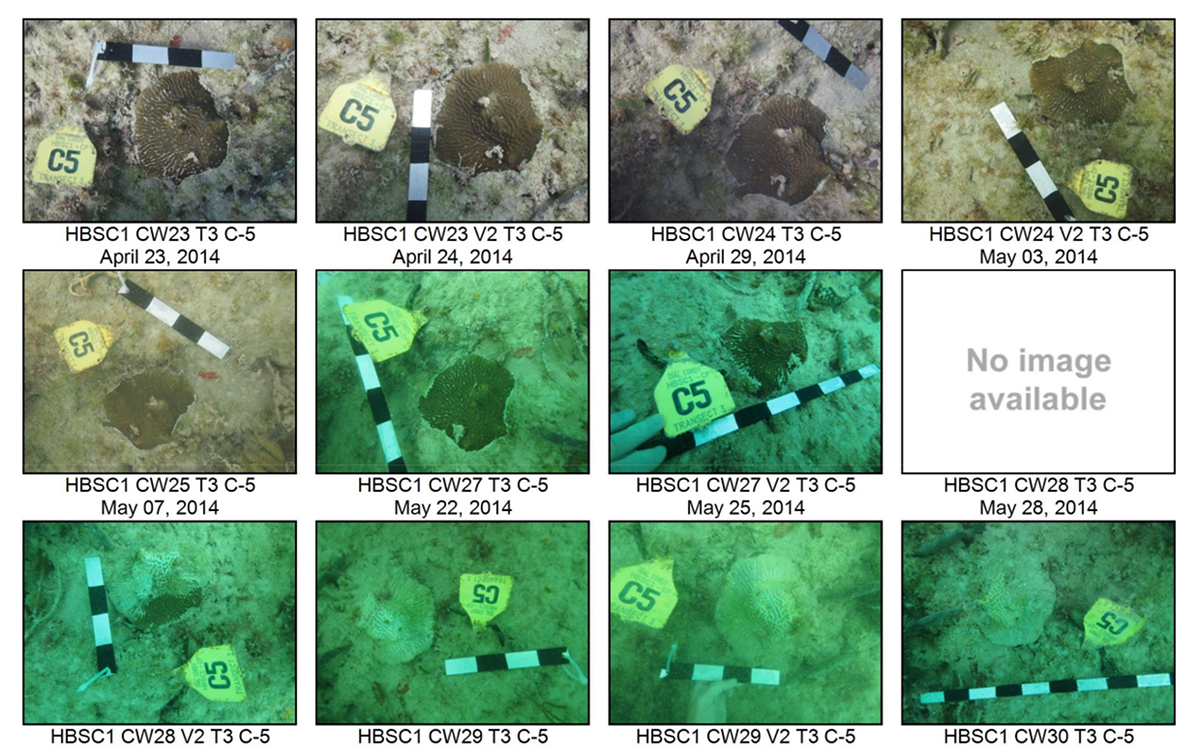
\includegraphics[width=\textwidth]{figures/hbsc1_cp.png}
	\caption{Lightroom photos of tagged corals at site HBSC1-CP \citep{dial2017}. The first signs of the disease appeared between May 25 and May 30. By June 4, the whole colony was completely dead}
\end{figure}
\newpage
\section{Model validation agains tide gauge observations}\label{onset:validation}
\begin{figure}[h!]
    \centering
	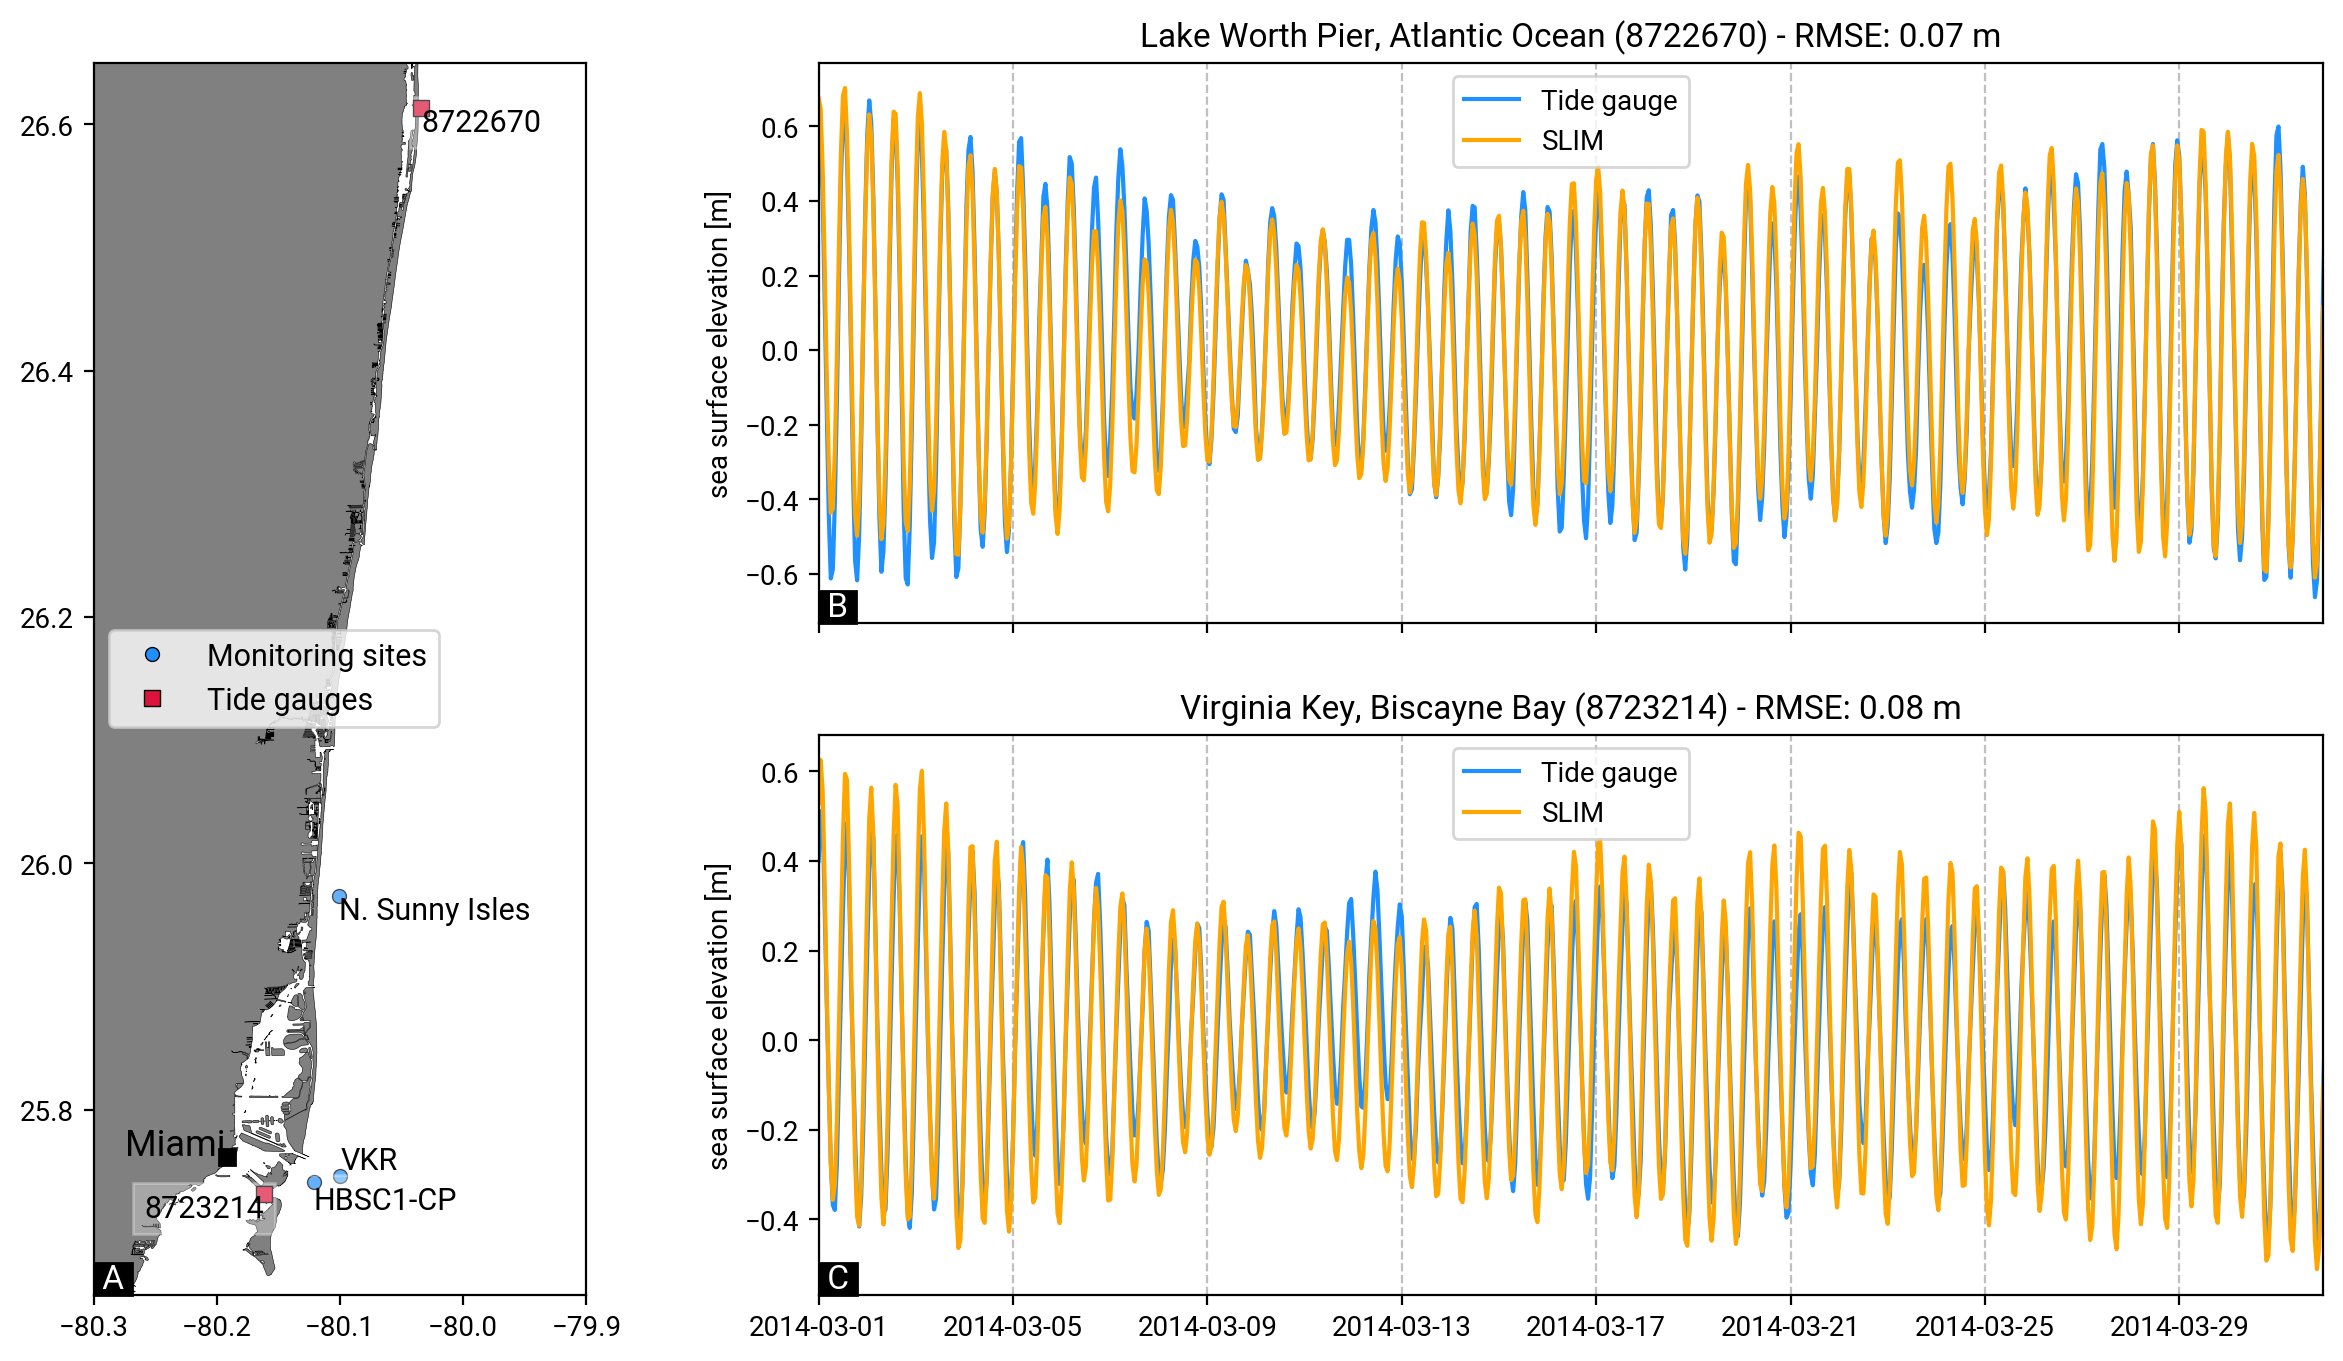
\includegraphics[width=\textwidth]{figures/fig_validation_new.png}
    \caption{\textbf{A}: Locations of the tide gauge stations (width IDs 8722670 and 8723214) from the National Data Buoy Center used to validated the modeled hydrodynamics. \textbf{B+C}: Comparison of the modeled sea surface elevation against tide gauge measurements in March 2014. The model Root Mean Square Error (RMSE) was below 10 cm at both stations.
}\end{figure}

\end{document}
\endinput
